% !TEX root = thesis-ex.tex
This section shall discuss the theoretical background necessary to understand jet measurements. It will discuss the fundamentals of quantum chromodynamics (QCD), the heavy ion collision system and the quark gluon plasma that is formed, and finally jets and jet energy loss. 

\section{Quantum Chromodynamics}
\label{sec:qcd}
% !TEX root = thesis-ex.tex
Quantum Chromodynamics is a gauge theory with SU(3) symmetry that describes the dynamics of the strong interactions between quarks and gluons.
It is part of the Standard Model \cite{Gaillard:1998ui}, the building blocks of which are shown in Figure~\ref{fig:sm_particles}.

%The Standard Model (SM) \cite{Gaillard:1998ui} describes the interactions between elementary particles that are listed in Figure~\ref{fig:sm_particles}.It is one the most successful theories in physics and describes three of the four fundamental forces of nature.These are the strong interaction, the weak interaction, and the electromagnetic interaction.A quantum theory for gravity is not part of the SM.

\begin{figure}[htbp]
\begin{center}
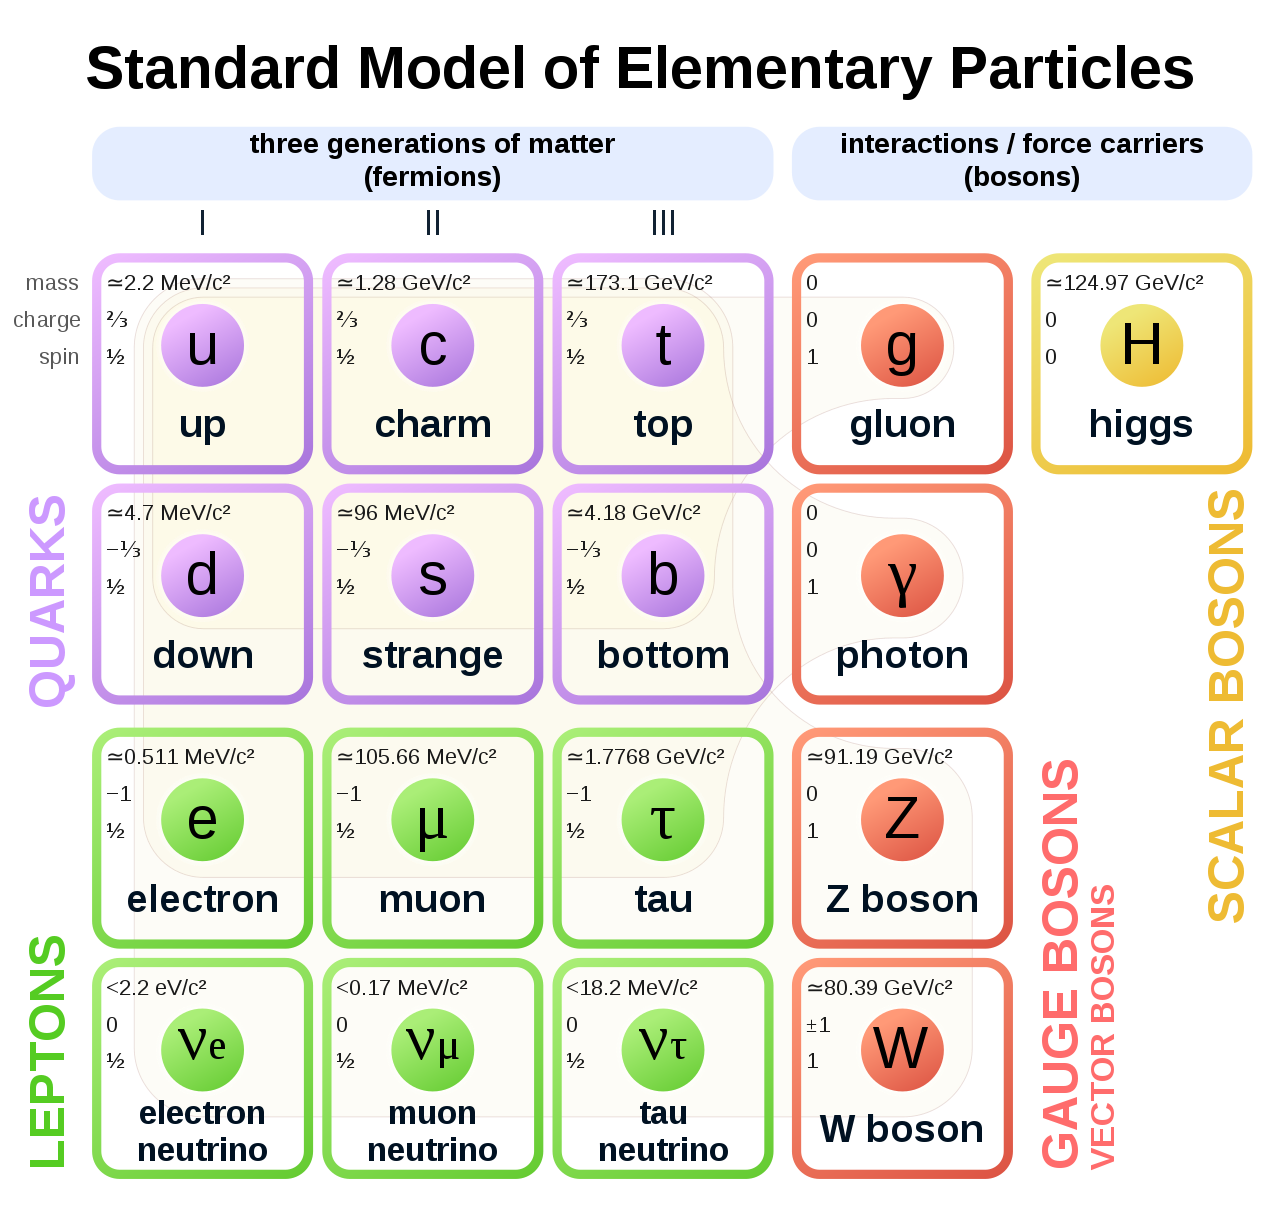
\includegraphics[width=0.5\textwidth]{figures/theory/SM}
\caption{The elementary particles of the standard model.
Figure taken from Ref.~\cite{SMpict}.}
\label{fig:sm_particles}
\end{center}
\end{figure}

%Within the SM, the dynamics of the strong interactions involving quarks and gluons are described by Quantum Chromodynamics (QCD), 

Quarks are fermions with a spin of $1/2$, and carry a fractional electric charge as well as a color charge.
They all have mass and come in six flavors: up, down, strange, charm, top, bottom.
The lightest quarks (u and d) combine and form stable particles, while the heavier quarks can only be produced in energetic environments and decay rapidly.
Gluons are gauge bosons (force carriers) with a spin of $1$, and are what hold quarks together.
The dynamics of the quarks and gluons, collectively referred to as partons are described by the QCD Lagrangian given by \cite{Beringer:1481544}:

\begin{align}
\mathcal{{L}}_{\mathrm{QCD}} = \sum_q \bar{\psi}_{q,a} (i \gamma^\mu \partial_\mu \delta_{ab} - g_s \gamma^\mu t_{ab}^C \mathcal{A}_\mu^C - m_q \delta_{ab}) \psi_{q,b} - \frac{1}{4} F_{\mu\nu}^A F^{A \mu\nu}
\end{align}
where $\psi_{q,a}$ and $\psi_{q,b}$ are quark-field spinors for a quarks with flavor $q$, mass $m_q$, and color $a$ and $b$ respectively, with the values for $a$ and $b$ ranging  from 1 to 3 (for the three colors).
The $\mathcal{A_\mu^C}$ corresponds to the gluon field with $C$ taking values from 1 through 8 (for the 8 types of gluons).
The $t_{ab}^C$ corresponds to the Gell-Mann matrices that are the generators of the SU(3) group, and dictate the rotation of the quarks color in SU(3) space when it interacts with a gluon.
The coupling constant is encoded within $g_s$, which is defined by $g_s \equiv \sqrt{4 \pi \alpha_s}$.
The field tensor $F_{\mu\nu}^A$ can be written in terms of the structure constants of the SU(3) group $f_{ABC}$, and is given by:

\begin{align}
F_{\mu\nu}^A = \partial_\mu \mathcal{A}_\nu^A - \partial_\nu \mathcal{A}_\mu^A - g_s f_{ABC} \mathcal{A}^B \mathcal{A}^C
\end{align}
While many parallels can be drawn between Quantum Electrodynamics (QED, the theory that describes photons and electrons) and QCD, the main difference between the two comes from the gluon-gluon interactions allowed in QCD, making it non-Abelian.
These interactions can be summarized as shown in Figure \ref{fig:qcd_diagrams}.

\begin{figure}[htbp]
\begin{center}
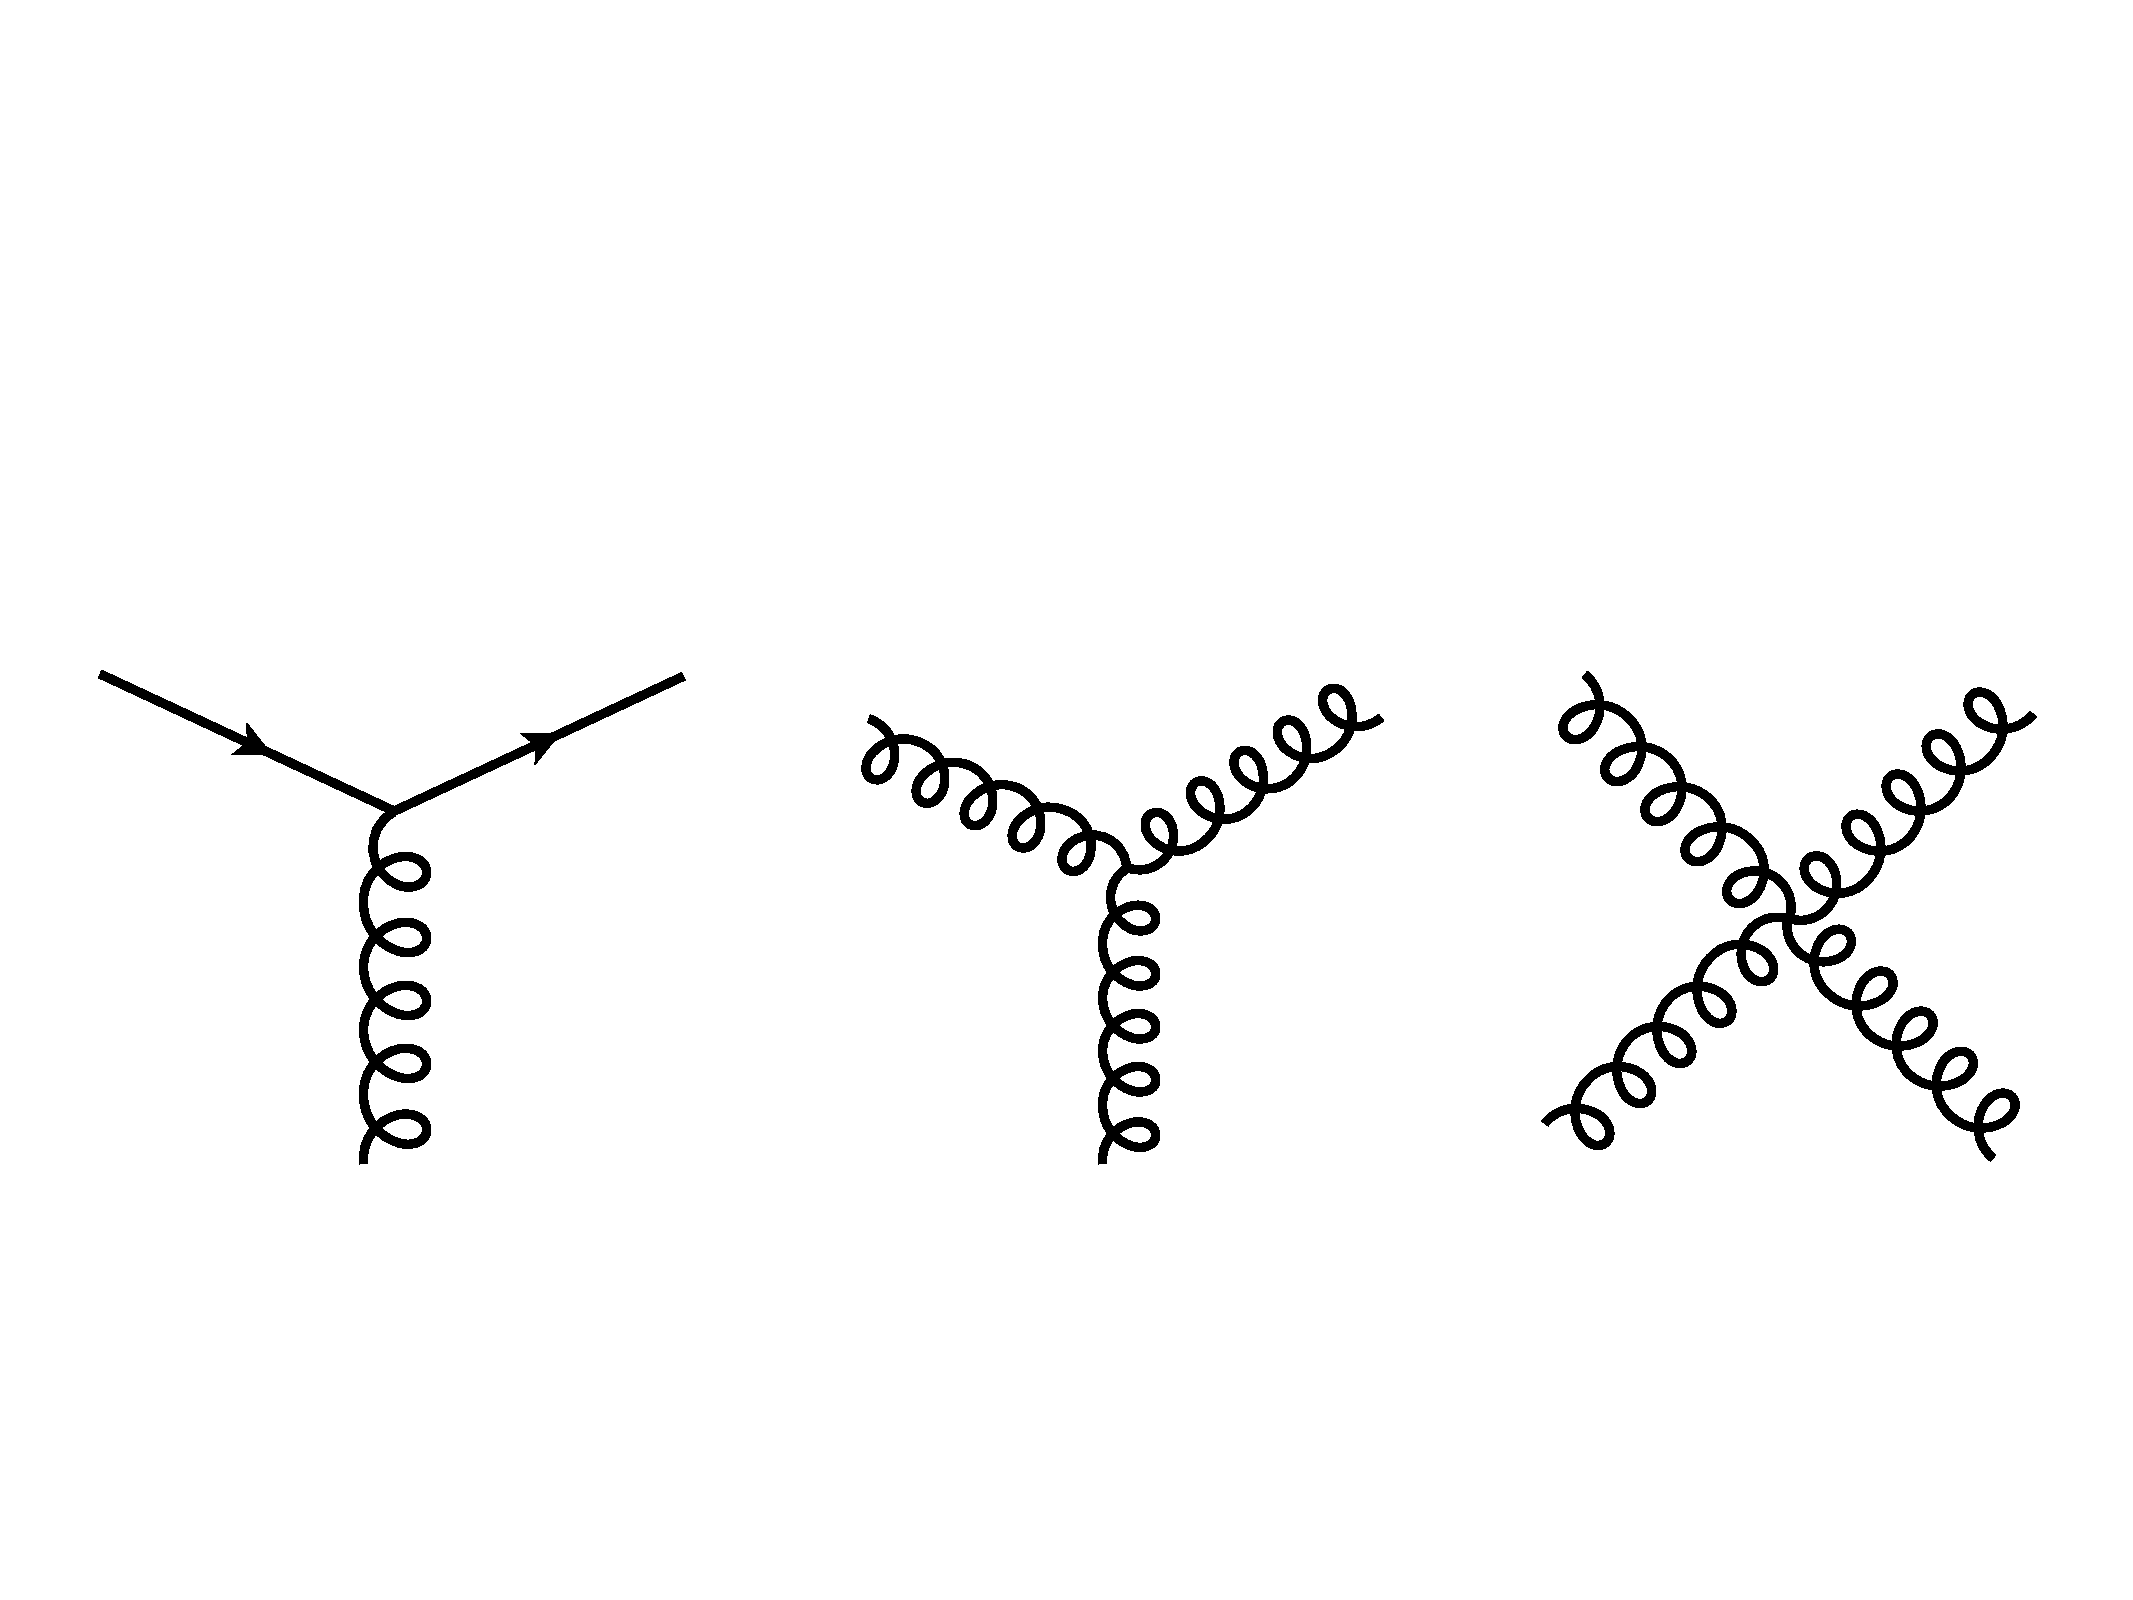
\includegraphics[width=0.8\textwidth]{figures/theory/qcd_diagrams}
\caption{The allowed vertices in QCD.
The vertices involving two or more gluons are unique to QCD and do not have a QED analog.}
\label{fig:qcd_diagrams}
\end{center}
\end{figure}

A core feature of QCD is that the coupling constant \alphas\ has an energy dependence shown in Figure~\ref{fig:running_coupling}.

\begin{figure}[htbp]
\begin{center}
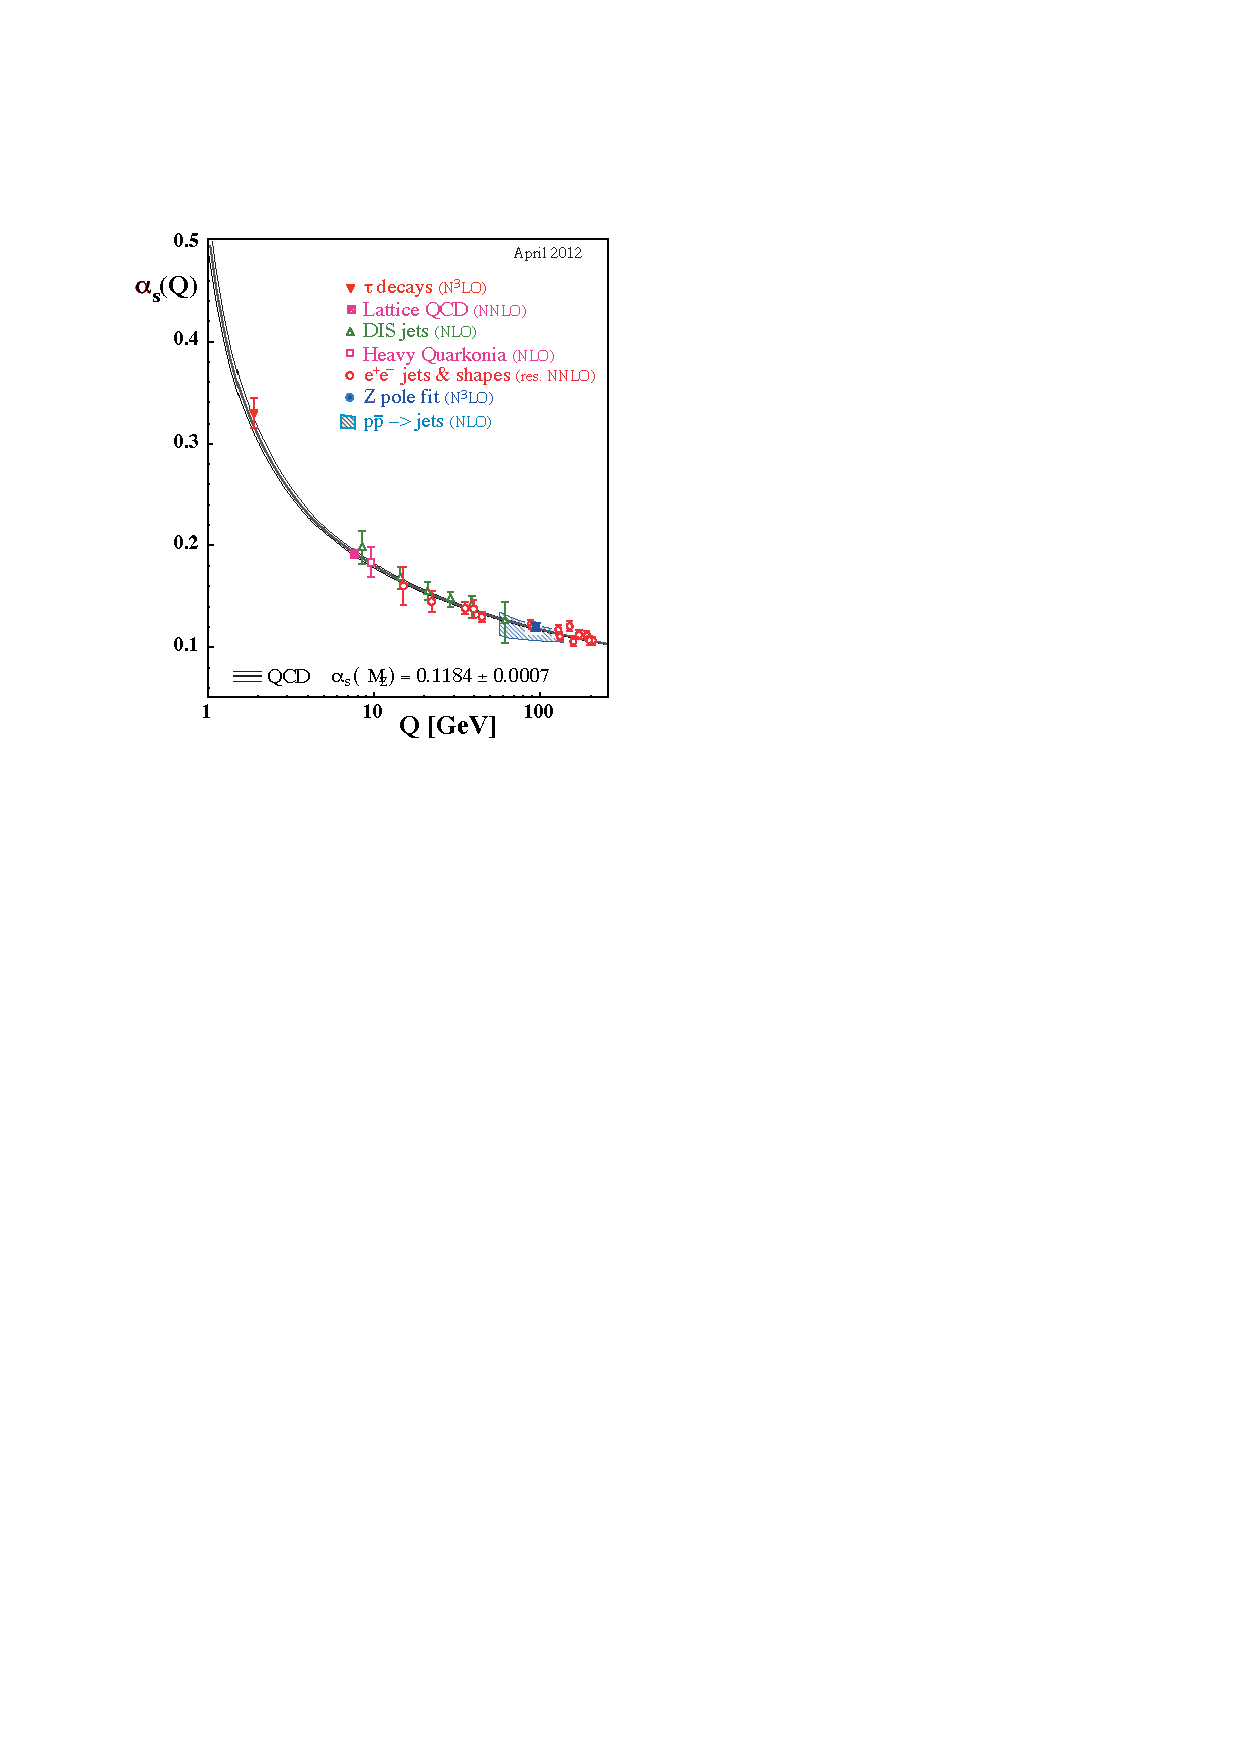
\includegraphics[width=0.5\textwidth]{figures/theory/running_coupling}
\caption{The running coupling constant $\alpha_s$ as a function of the momentum transfer $Q$.
Figure taken from Ref.~\cite{Beringer:1481544}.}
\label{fig:running_coupling}
\end{center}
\end{figure}

This dependence can be expressed in terms of the $\beta$ function as

\begin{align}
Q^2 \frac{\partial \alpha_s (Q^2)}{\partial Q^2} = \beta(\alpha_s (Q^2))
\end{align}
where $Q$ is the momentum transfer in the particle reaction
\footnote{The momentum transfer $Q$ is the amount of momentum transferred in a scattering process.}.
The beta function can be expressed using perturbative QCD (pQCD) as:

\begin{align}
\beta( \alpha_s ) = - (b_0 \alpha_s^2 + b_1 \alpha_s^3 + b_2 \alpha_s^4...)
\end{align}
where the coefficients $b_i$ depend on the number of colors and flavors.
This running coupling constant is small and asymptotically tends to zero at large energy scales (or at small distances) and is large at small energy scales (large distances).
This running coupling phenomenon leads to two key behaviors: asymptotic freedom and color confinement.


\subparagraph{Asymptotic Freedom: }
At high energy scales (small distances), the QCD coupling constant $\alpha_s$ is small and tends to zero, implying a free particle behavior of quarks and gluons\cite{PhysRevLett.30.1343, PhysRevD.8.3633}.
This has been observed by a variety of deep inelastic scattering (DIS) experiments \cite{Deur:2014vea, Kim:1998kia, Altarelli:1996nm, RevModPhys.63.597, Kataev:2001kk, Alekhin:2012ig, Alekhin:2013nua, Blumlein:2006be, Aaron:2007xx, Chekanov:2007pa, Chekanov:2008af, Abramowicz:2010cka, Abramowicz:2010ke, Aaron:2009vs}.
These scattering experiments shown in Figure~\ref{fig:dis_schematic}, probe the interior of a nucleon using highly energetic leptons like electrons. The electron scatters off of the target proton, producing a lepton and a hadron shower. Bu 
First done by MIT-SLAC \cite{PhysRevLett.23.930, PhysRevLett.23.935}, these DIS experiments showed the weak $Q^2$ dependence on the inelastic scattering cross-sections, as well as Bjorken scaling \cite{PhysRev.179.1547}, where the proton structure functions are independent of the momentum transfer.
These experiments revealed the point-like constituents of the proton and paved the road to an asymptotically free theory.

\begin{figure}[htbp]
\begin{center}
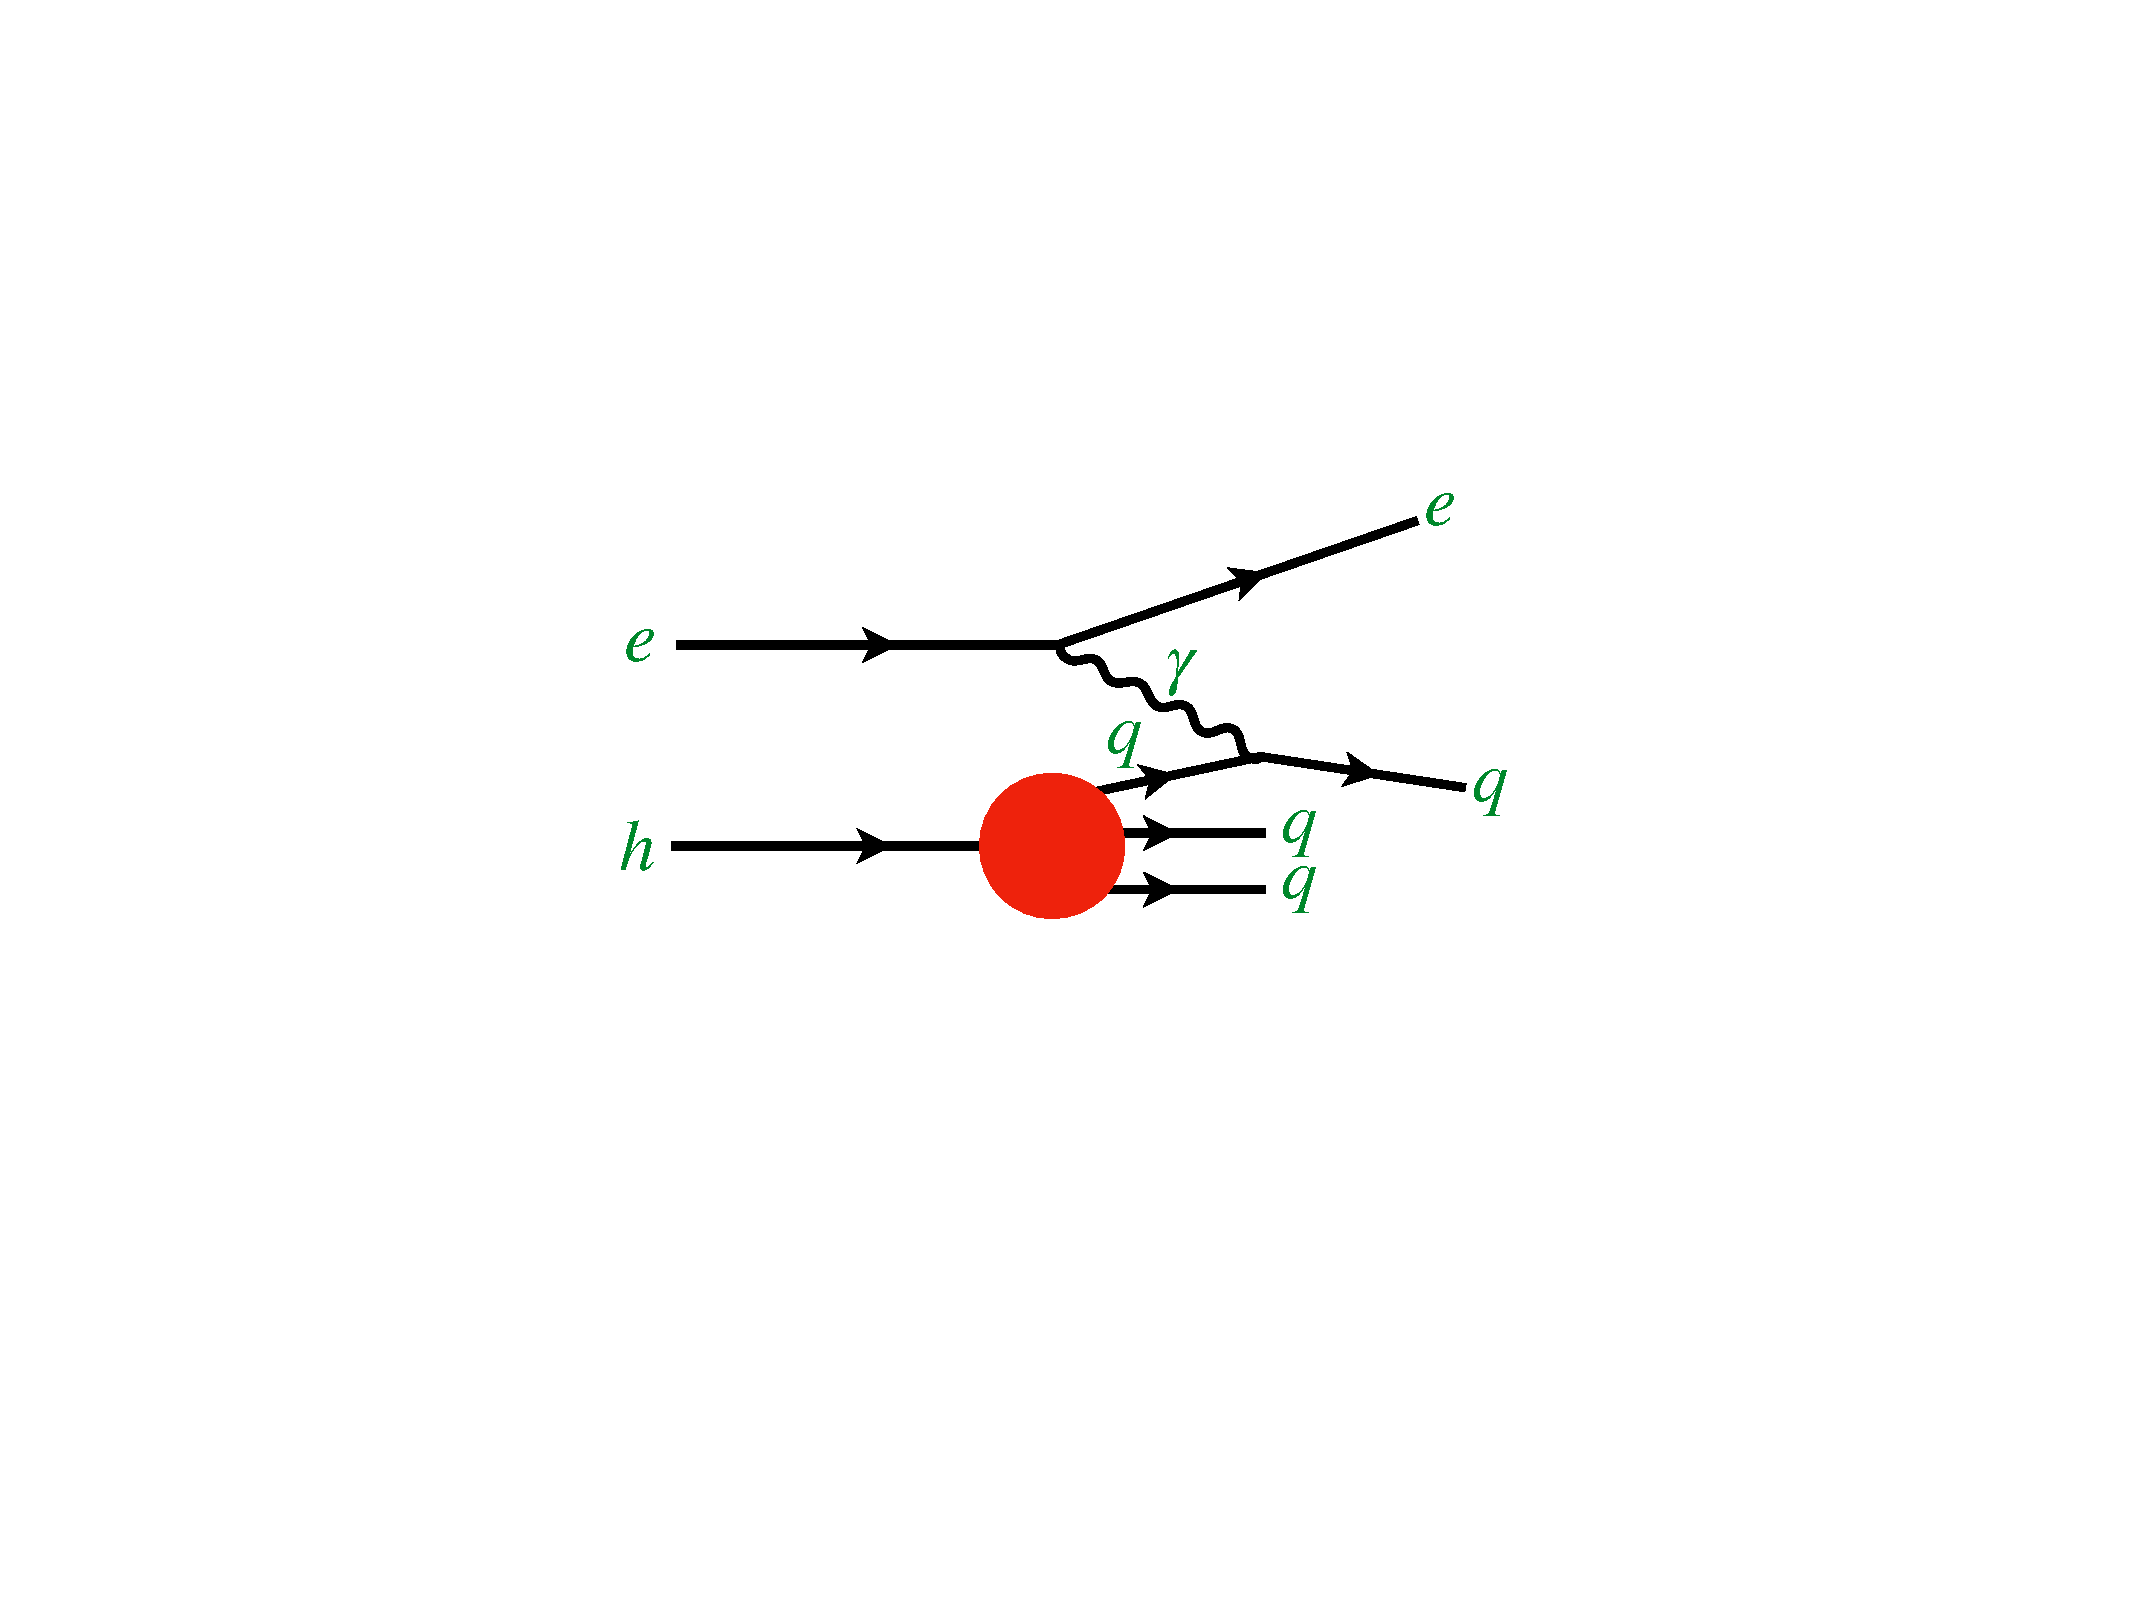
\includegraphics[width=0.35\textwidth]{figures/theory/DIS}
\caption{Schematic of the deep inelastic scattering experiment.}
\label{fig:dis_schematic}
\end{center}
\end{figure}


\subparagraph{Color Confinement}
The opposite end of the running coupling constant phenomenon is color confinement.
Proved to be a consequence of asymptotic freedom in Ref~\cite{Nishijima1996}, this property of QCD described in Ref.~\cite{PhysRevD.10.2445} forbids the direct observation of free quarks and gluons, allowing only for composite particles that are color singlets.
While have been numerous efforts to understand the source of this phenomenon like in Refs.~\cite{BUCHMULLER1982479, KOGUT1976199, PhysRevD.31.2910, PhysRevD.57.2603, PhysRevD.62.114503, RevModPhys.55.775, PhysRevLett.90.102001}, these are based on numerical calculations.
An analytic proof of color confinement still escapes description and in fact, is one of the Millennium Problems \cite{MillenniumProb}.


%\subsection{Parton Distribution Functions}
%Deep ineslatic scattering experiments showed the internal point-like structure of a proton that can be described in terms of probability density functions called parton distribution functions.
%These are written in terms of the longitudinal momentum fraction carried by a constitutent proton, $x$, given as:
%
%\begin{align}
%x = \frac{Q^2}{2 P \dot q} = \frac{Q^2}{2 M \nu}
%\end{align}
%where $\nu$ is the energy of the photon shown in Figure~\ref{fig:dis_schematic}. This can be determined by 




%An analytic proof of the origin of color confinement is described in Ref.\cite{Gao:2018xsg}.
%==========================================================
%
%%QCD allows for predicting a variety of observables in particle reactions involving quarks and gluons in terms of the coupling constant $\alpha_s$.
%QCD amplitudes can be calculated by using the matrix elements for the basic diagrams shown in Figure~\ref{fig:qcd_diagrams} along with the quark and gluon propagators.Perturbative calculations done with the assumption that the coupling constant \alphas $ < 1 $ allow for 
%Another major feature 
% quark and gluon propagators along with teh corre
%
%
%

%The classical QCD Lagrangian is given by \cite{Chyla:2004zz}
%
%\begin{align}
%\mathcal{{L}}_{\mathrm{QCD}} = \sum_q \bar{\psi}_{q,a} (i \gamma^\mu \partial_\mu \delta_{ab} - g_s \gamma^\mu t_{ab}^C \mathcal{A}_\mu^C - m_q \delta_{ab}) \psi_{q,b} - \frac{1}{4} F_{\mu\nu}^A F^{A \mu\nu}
%\end{align}
%
%%\begin{align}
%%\mathcal{{L}}_{\mathrm{QCD}} &= \mathcal{L}_g + \mathcal{L}_q \\
%%&=  -\frac{1}{4} F_{\mu\nu} F^{\mu\nu} + \bar{\Psi}(i  \slashed{\partial} - m_q) \Psi + g \bar{\Psi} \gamma_\mu T \Psi A^\mu
%%\end{align}
%
%\begin{align}
%\mathcal{{L}}_{\mathrm{QCD}} =  -\frac{1}{4} F_{\mu\nu} F^{\mu\nu} + \bar{\Psi}(i  \slashed{\partial} - m_q) \Psi + g \bar{\Psi} \gamma_\mu T \Psi A^\mu
%\end{align}
%
%\begin{align}
%F^{\mu\nu}_a (x) \equiv \frac{\partial A_a^\nu (x)}{\partial x_\mu} - \frac{\partial A_a^\mu (x)}{\partial x_\nu}
%\end{align}
%
%%This Lagrangian is can be thought of as the sum of the quark and gluon terms $\mathcal{L}_g$ and $\mathcal{L}_q$, where
%%\begin{align}
%%\mathcal{L}_g &= - \frac{1}{4}\frac{1}{4} F_{\mu\nu} F^{\mu\nu} 
%%\end{align}
%
%
%where $Q$ is the momentum transfer in the particle reaction.This running coupling constant is small and asymptotically tends to zero at large energy scales (or at small distances) and is large at small energy scales (large distances).This can be seen in Figure \ref{fig:running_coupling}, which shows the $\alpha_s$ dependence on $Q$.This running coupling leads to two key behaviors discussed below.
%
%
%
%

\section{Heavy Ion Collisions}
\label{sec:HICollisions}
% !TEX root = thesis-ex.tex
Heavy ion collisions can be used as a tool to study the Quark Gluon Plasma \cite{SHURYAK198071} . They provide access to the otherwise confined partons, and give insight into the QCD phase diagram and the transition between the QGP and hadronic matter. 

In a heavy ion collision, the colliding nuclei are accelerated to relativistic energies and are Lorentz contracted discs. In the case of a \pbpb\ collision the relativistic $\gamma$ factor is between 100 and 2500 for beam rapidities of $y = 5.3$ and 8.5. Each nucleus contains many colored quarks and antiquarks, with three more quarks than anti-quarks per nucleon, with the $q\bar{q}$ popping in and out of the vacuum due to quantum fluctuations. These $q\bar{q}$ pairs are sources of transverse color fields and the corresponding force carriers, the gluons. 

When these pancake like discs collide, their color fields interact and there is a color charge exchange, producing longitudinal color fields that fill the space between the receding discs. While the maximum energy density in the process occurs just at the collision, the energy density 1 fm/c after the collision is 12 $\mathrm{GeV} / \mathrm{fm}^3$, much higher than the 500 $\mathrm{MeV} / \mathrm{fm}^3$ in a typical hadron. Lattice QCD calculations in thermodynamics show that at these energies, the partons produced in the collision cannot be treated as a collection of distinct hadrons. 
%In fact, these partons are strongly coupled to each other and form a medium called the Quark Gluon Plasma (QGP) \cite{???}. 

%In a heavy ion collision, the experimenter can only tune the size of the colliding nuclei, and the energy that they are being collided at. There is no experimental control over the impact parameter or the structure functions that dictate the momentum distribution of nucleons within the nucleus. These have to be determined event by

% most of the partons are participate in soft interactions that do not involve large transverse momentum transfer, and are hence scattered only at small angles. A small fraction of the colliding partons however do undergo hard perturbative interactions and lead to particles with large transverse momenta.
%These subsequently decaying to $q\bar{q}$ pairs. 
%The QGP can be described by relativistic hydrodynamics, and has a viscosity to entropy ratio that is almost at the theoretical minimum of of $\eta / S = 1/4\pi$ \cite{5,6, check126}. 

After the collision the energy density between the receding nuclei starts to decrease as the QGP cools and expands. This process, seen in Figure~\ref{fig:qgp_form}, continues till the energy density drops to below that within a hadron and the fluid ``hadronizes''. These individual hadrons briefly scatter off of each other before they freely fly towards the detector (freeze-out).

%Once formed, the QGP flows hydrodynamically, with the initial pressure driving the expansion and the subsequent cooling. 
% It is to be noted that there is QGP continuously formed in the wake of the nuclei since the partons produced at large rapidities are highly relativistic and 

\begin{figure}[htbp]
\begin{center}
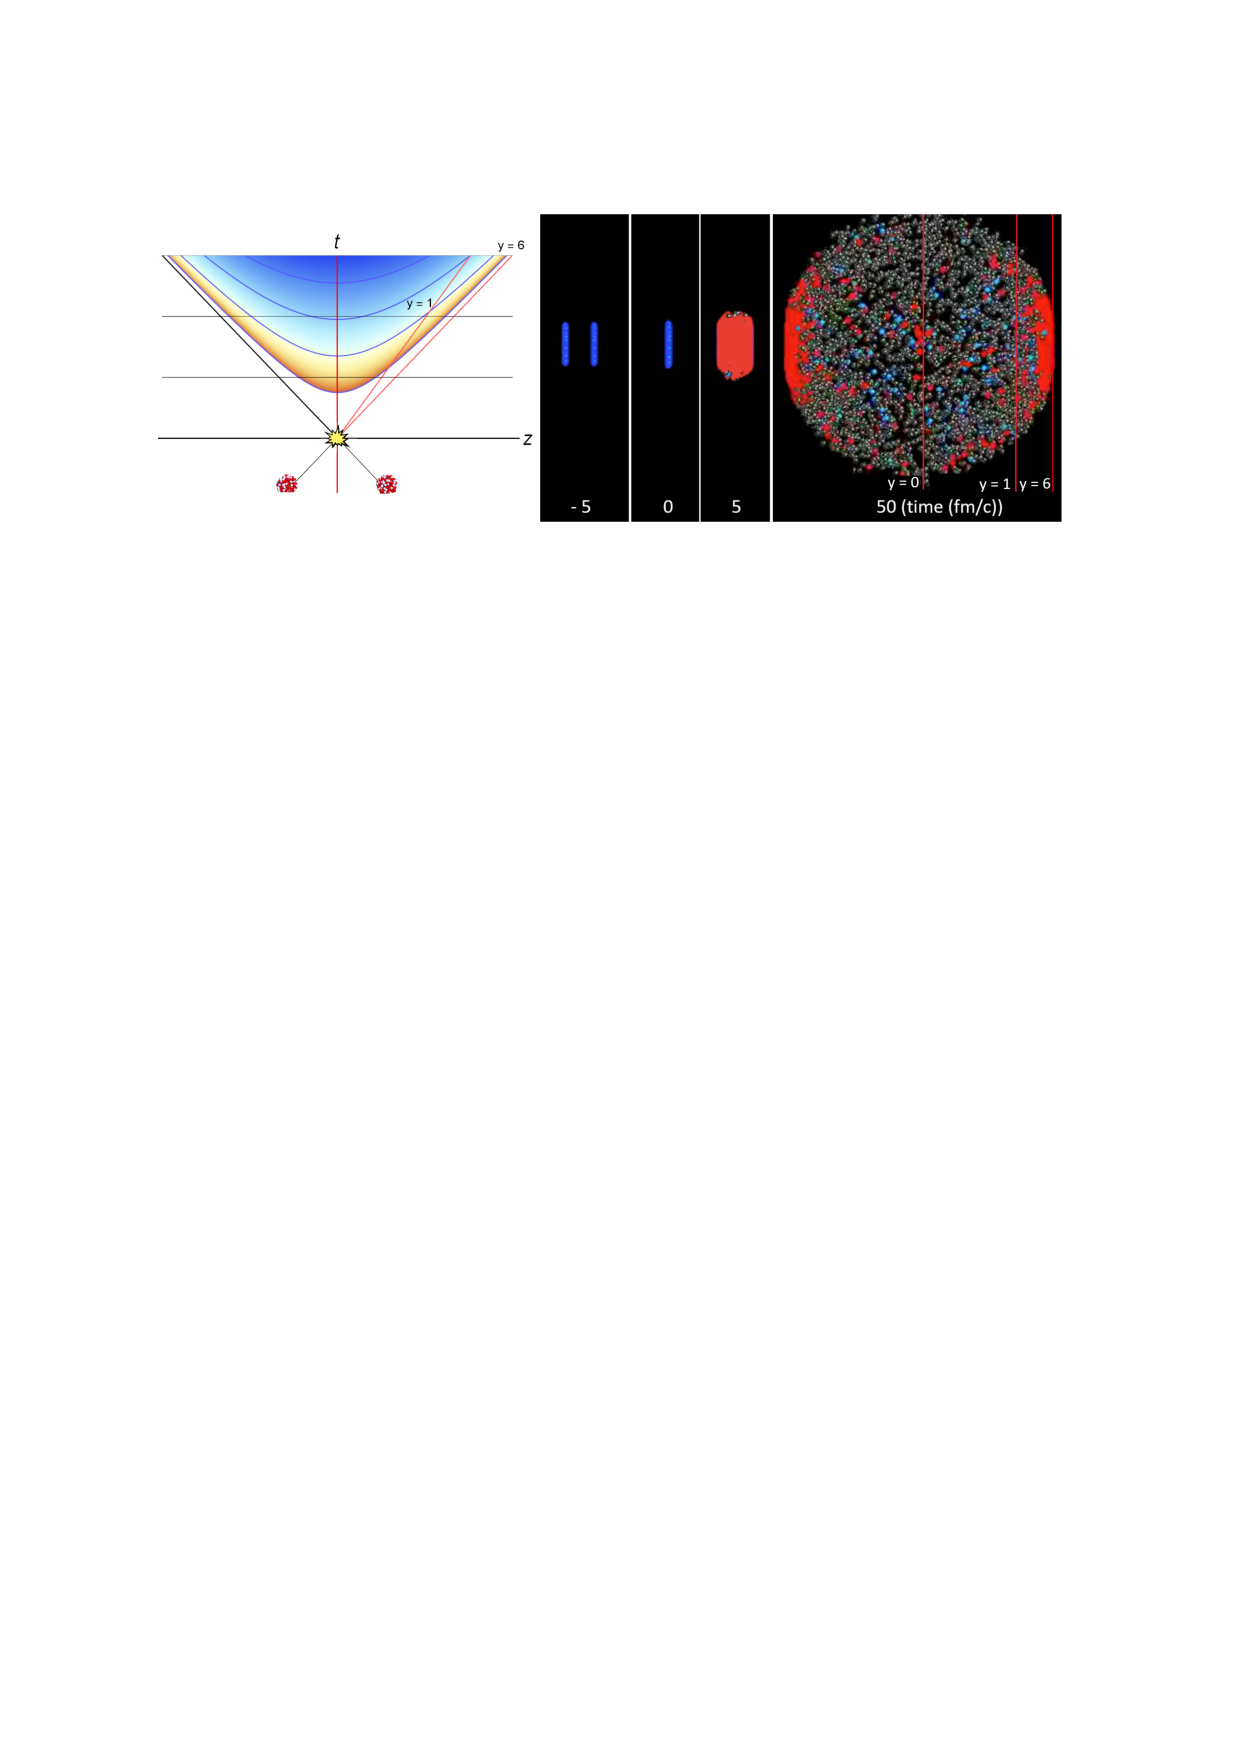
\includegraphics[width=0.85\textwidth]{figures/theory/qgp_formation}
\caption{(left) Space-time diagram for a heavy ion collision. The color is indicative of the temperature of the QGP formed. (right) Snapshots of a heavy ion collision at $\sqrtsnn = 2.76$ TeV at different times. The Lorentz contracted nuclei are in blue while the QGP is in red. Figure from Reference \cite{Busza:2018rrf}.  }
\label{fig:qgp_form}
\end{center}
\end{figure}

While Figure~\ref{fig:qgp_form} shows snapshots of a head on (central) collision between two large nuclei, it is possible to have collisions where the impact parameter is larger and hence the overlap region is smaller. These collisions, called peripheral collisions, qualitatively undergo the same process described above, with the size and shape of the QGP being different.

% In fact, peripheral collisions are very similar to proton-proton collisions, with differences coming mainly from nuclear PDFs.

The basic parameters of a heavy ion collision such as the number of participants \Npart\ and number of binary collisions \Ncoll\ can be determined using the Glauber Monte Carlo simulations \cite{glauberArticle, glauberMisc}. This technique considers a nucleus-nucleus collision as a collection of independent binary nucleon-nucleon collisions; the colliding nuclei are modeled as a set of uncorrelated nucleons being positioned within the nucleus based on a the nuclear density function uniform in azimuthal and in polar angles. The nuclear density function shown in Figure~\ref{fig:nuclearDensity} for Au and Cu, is given by:

\begin{align}
\rho(r) = \rho_0 \frac{1 + w (r/R)^2}{1+e^{\frac{r-R}{a}}}
\end{align}
where $\rho_0$ is the nucleon density, $R$ is the nuclear radius, $a$ is the skin depth, $w$ corresponds to deviations from a circular shape and is typically zero for larger nuclei like Cu, W, Au, Pb, and U. For the Pb nuclei used at the LHC, $w = 0$, $R = 6.62$ fm and $a =0.55$ fm \cite{DEVRIES1987495}. 

\begin{figure}[htbp]
\begin{center}
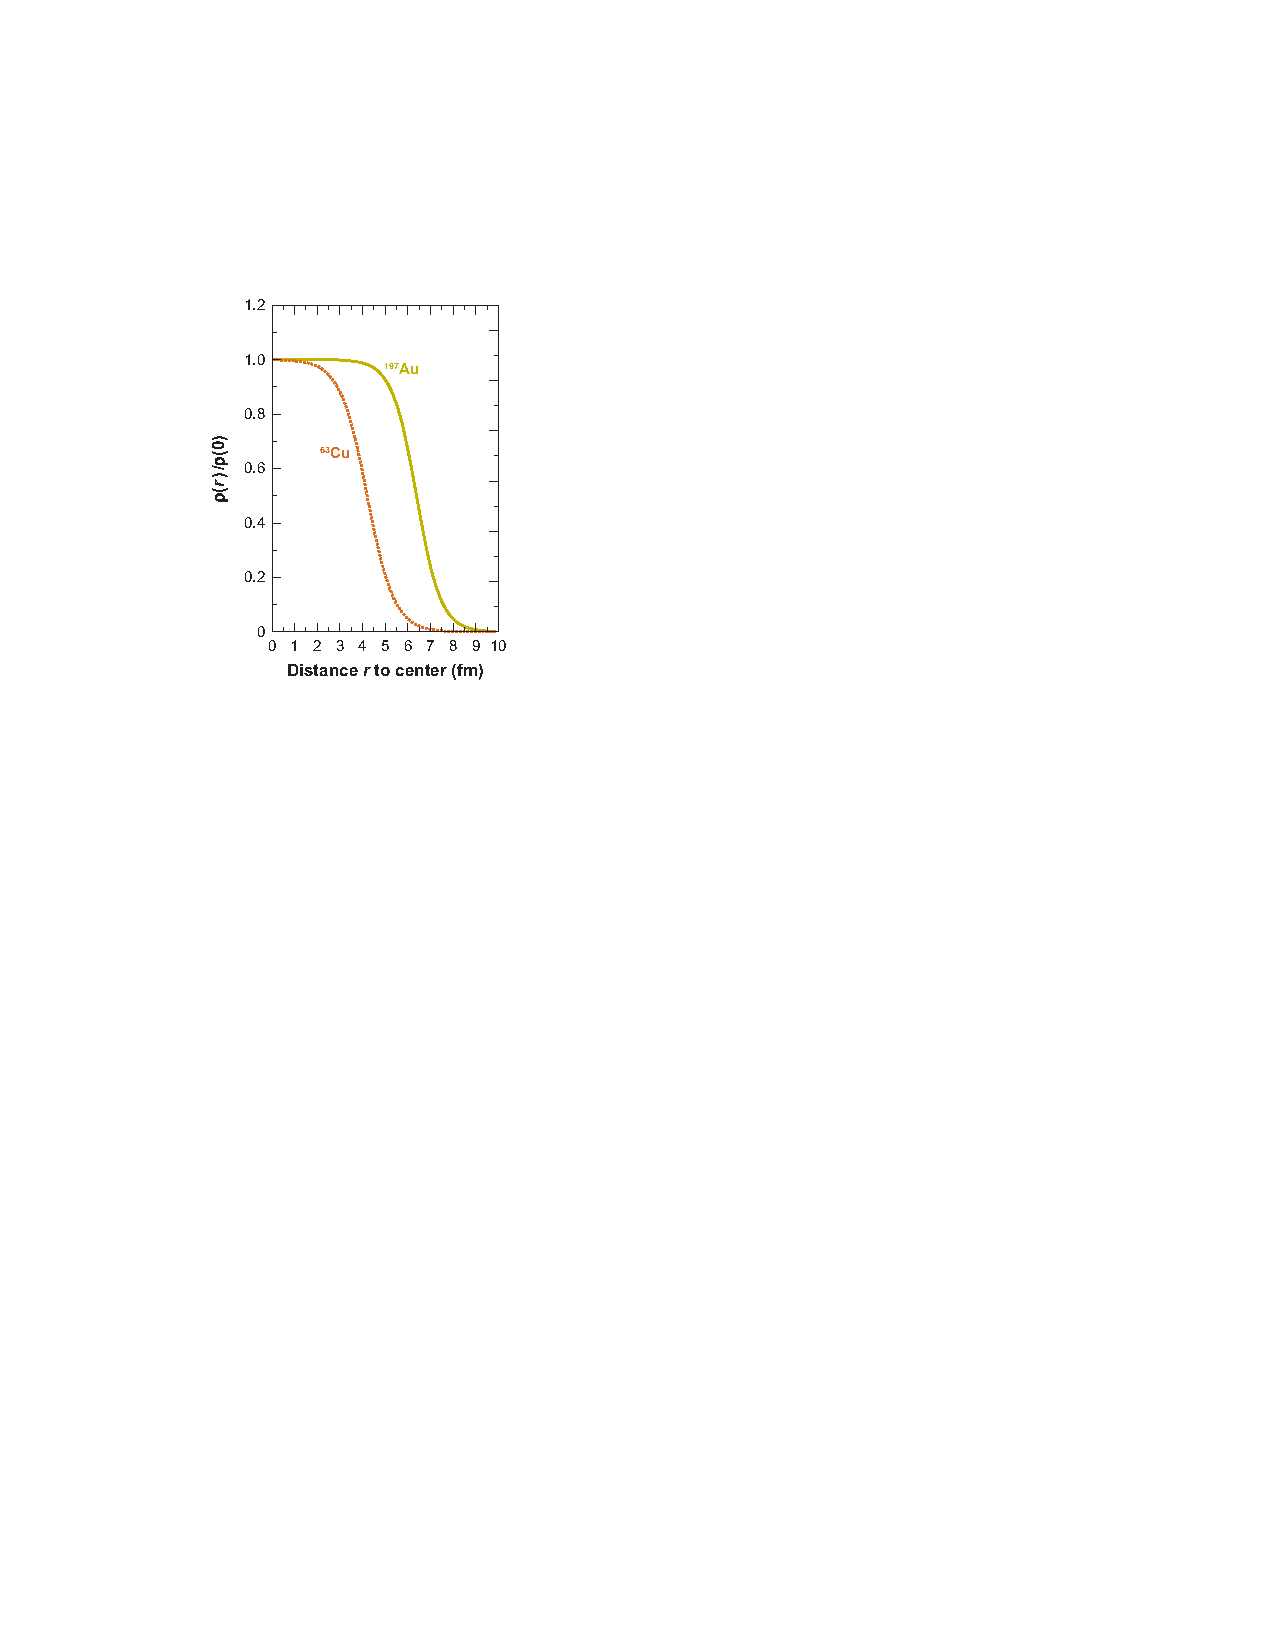
\includegraphics[width=0.45\textwidth]{figures/theory/nuclearDensity}
\caption{ The nuclear density distributions for nuclei used at RHIC: Cu ($w = 0$, $R = 4.2$ fm and $a =0.48$ fm)  and Au ($w = 0$, $R = 6.38$ fm and $a =0.535$ fm) \cite{doi:10.1146/annurev.nucl.57.090506.123020, DEVRIES1987495}.}
\label{fig:nuclearDensity}
\end{center}
\end{figure}

They are then arranged with a random impact parameter $b$ based on the distribution $d\sigma/d b = 2\pi b$ and projected onto the $x-y$ plane as shown in Figure~\ref{fig:glauberMC}. They are then made to travel on straight trajectories, colliding if $d \leq \sqrt{\sigma_{\mathrm{inel}}^{\mathrm{NN}}/ \pi}$, where $d$ is the distance between the nucleons in a plane transverse to the beam axis and $\sigma_{\mathrm{inel}}^{\mathrm{NN}}$ is the inelastic scattering cross section. \cite{doi:10.1146/annurev.nucl.57.090506.123020, Alver:2008aq}

\begin{figure}[htbp]
\begin{center}
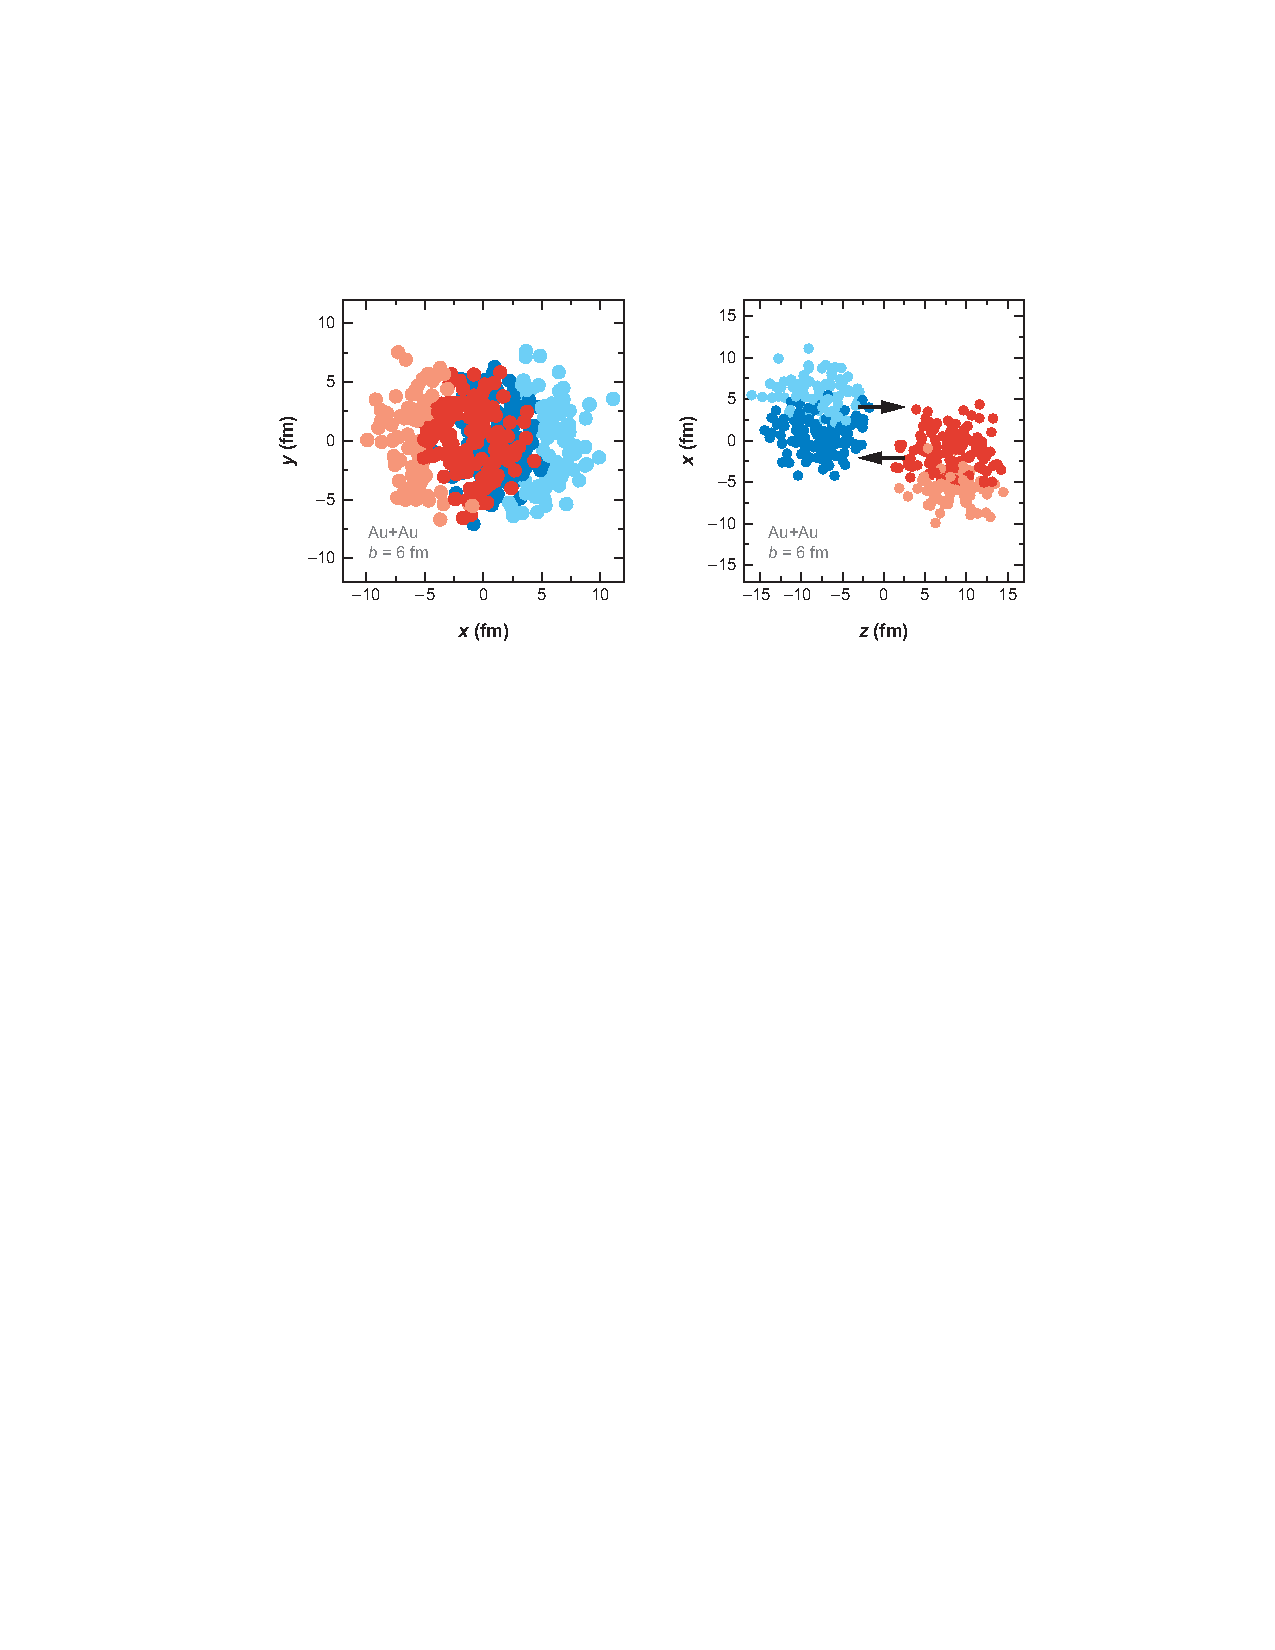
\includegraphics[width=0.85\textwidth]{figures/theory/glauberMC}
\caption{A Glauber Monte Carlo event for $Au+Au$ at \sqrtsnn = 200 geV with impact parameter of 6 fm viewed in the (left) transverse plane and (right) along the beam axis. Darker circles represent the participating nucleons. Taken from \cite{doi:10.1146/annurev.nucl.57.090506.123020}. }
\label{fig:glauberMC}
\end{center}
\end{figure}



An important parameter for colliding nuclei A and B with $A$ and $B$ nucleons is the thickness function $T_{AB}$. It describes the effective overlap area in which specific nucleons in the two colliding nuclei can interact. It can be defined in terms of the probability per unit area of a given nucleon being located at a particular distance $s$ within the nucleus. For the colliding nuclei $A$ and $B$, this is given by $T_{A}({\bf{s}}) = \int \rho_A ({\bf{s}}, z_A) dz_{A}$ and $T_{B}({\bf{s}}) = \int \rho_B ({\bf{s}}, z_B) dz_{B}$. Then, $T_{AB}$ is given by

\begin{align}
T_{AB}({\bf b}) = \int T_{A} ({\bf s}) T_{B} ({\bf s-\bf b}) d^2 s
\end{align}

The probability of then having $n$ interactions between nuclei $A$ and $B$ is given by the binomial distribution:

\begin{align}
P(n, { \bf b}) = {{AB} \choose {n}} \Big[T_{AB}( {\bf b} ) \sigma_{\mathrm{inel}}^{\mathrm{NN}} \Big]^n \Big[ 1 - T_{AB}( {\bf b} ) \sigma_{\mathrm{inel}}^{\mathrm{NN}} \Big]^{AB-n}
\end{align}

where the first term is the number of combinations for finding $n$ collisions from $AB$ possibilities, the second term is the probability for having exactly $n$ collisions, and the last term the probability of $AB-n$ misses. Then the total probability of an interaction between A and B is 

%\frac{d^2  s\sigma_{\mathrm{inel}}^{\mathrm{AB}} } {d b^2}  \def % p p_{\mathrm{inel}^{AB} (b) = \sum_{n=1}^{AB} P(n, {\bf b}) = %1- \Big[ 1 - T_{AB}( {\bf b} ) \sigma_{\mathrm{inel}}^{\mathrm{NN}} \Big]^{AB-n}

\begin{align}
\frac{d^2  \sigma_{\mathrm{inel}}^{\mathrm{AB}} }{db^2} \equiv p_{\mathrm{inel}}^{\mathrm{AB}} (b) = \sum_{n=1}^{AB} P(n, {\bf b}) = 1- \Big[ 1 - T_{AB}( {\bf b} ) \sigma_{\mathrm{inel}}^{\mathrm{NN}} \Big]^{AB}
\end{align}

Then the total cross section is given by

\begin{align}
\sigma_{\mathrm{inel}}^{\mathrm{AB}} = \int_0^\infty 2\pi b db \Bigg[ 1- \Big( 1 - T_{AB}( {\bf b} ) \sigma_{\mathrm{inel}}^{\mathrm{NN}}  \Big)^{AB} \Bigg]
\end{align}

and \Ncoll\ and \Npart are given by \cite{Kharzeev:2000ph, Bialas:1976ed}

\begin{align}
\Ncoll (b) = & \sum_{n=1}^{AB} n P(n, b) =  AB \times T_{AB}(b) \sigmainel \\
\Npart (b) = & A \int T_A ({\bf s}) \Big[ 1 - \big(1-T_B ({\bf s - b}) \sigmainel \big)^B \Big] d^2 s \\
+ & B \int T_B ({\bf s-b}) \Big[ 1 - \big(1-T_A ({\bf s}) \sigmainel \big)^A \Big] d^2 s \nonumber
\end{align}

The correlation between \Ncoll\ and \Npart\ can be seen in Figure~\ref{fig:NcollNpart}

\begin{figure}[htbp]
\begin{center}
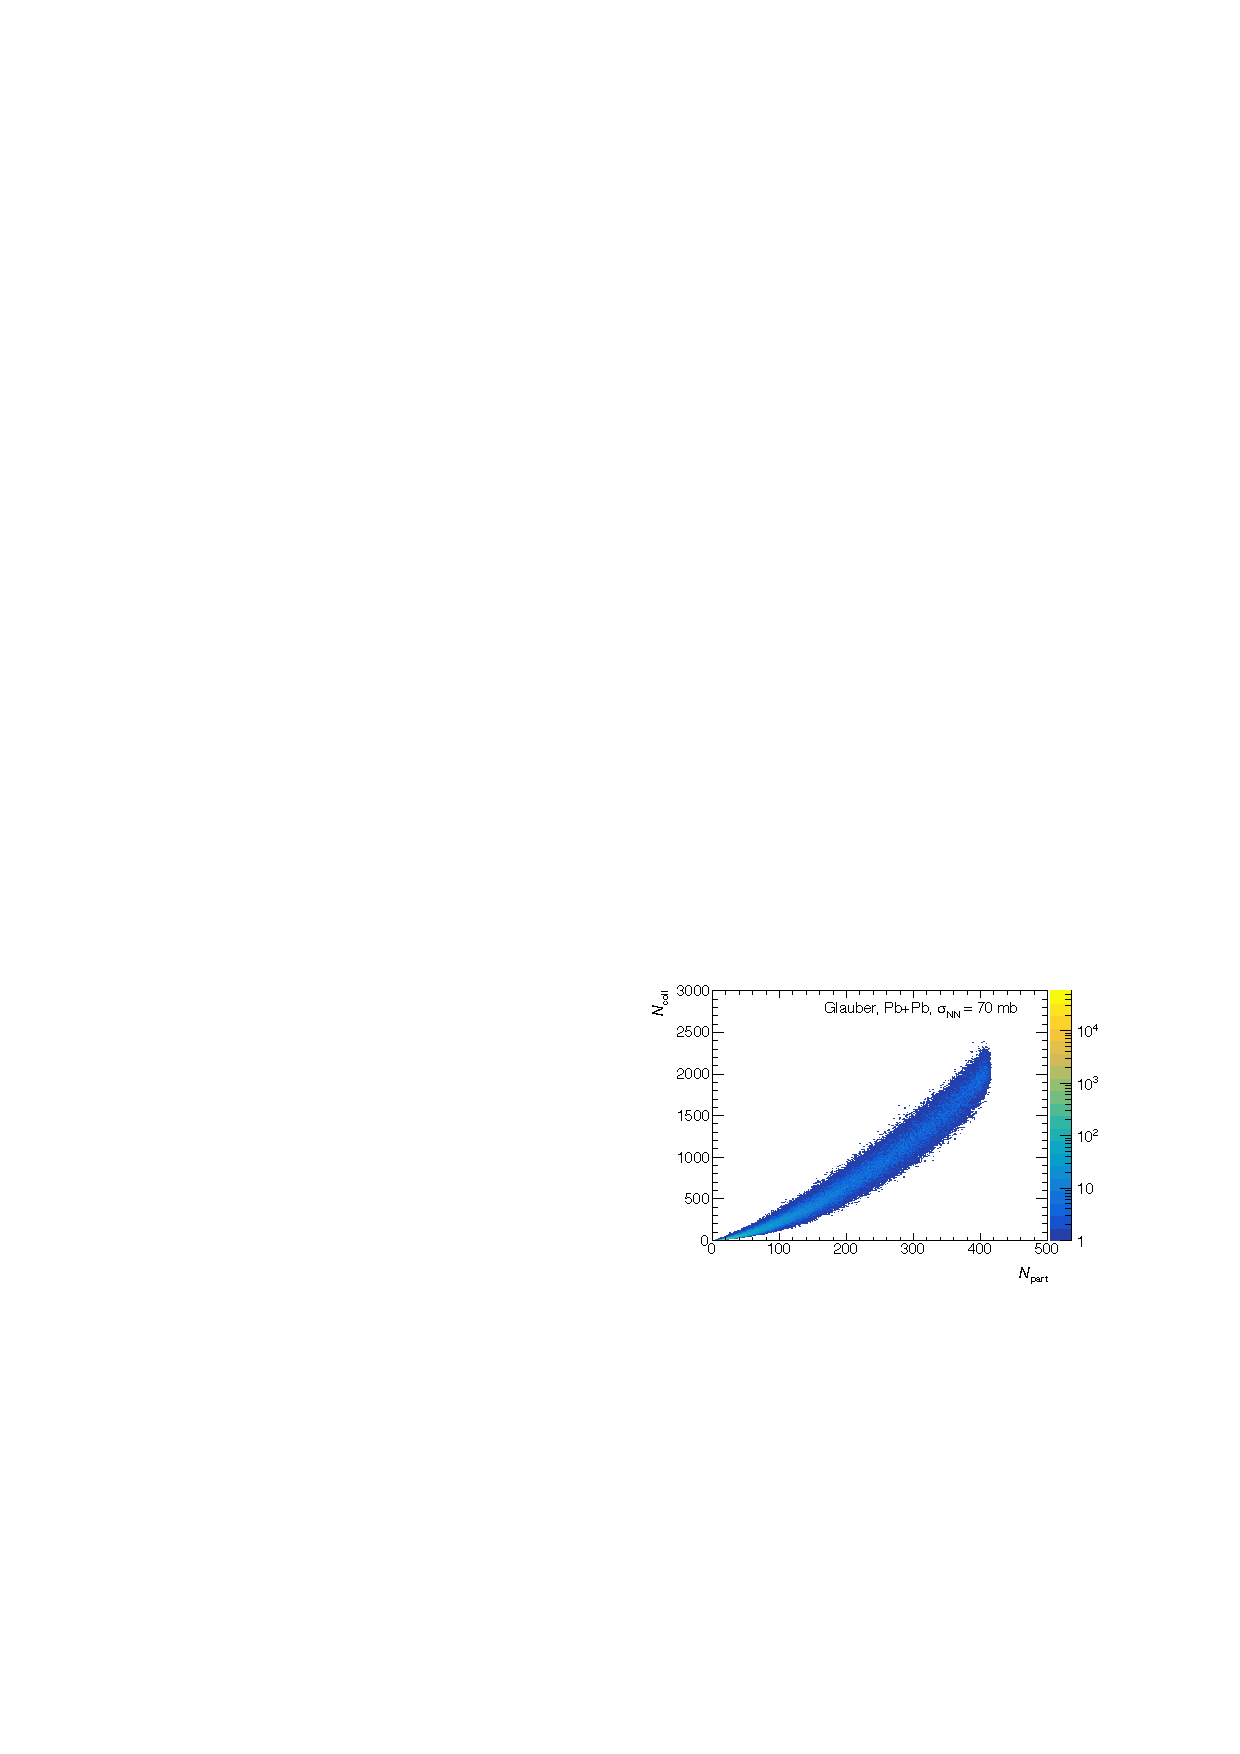
\includegraphics[width=0.55\textwidth]{figures/theory/NcollNpart}
\caption{The $\Ncoll-\Npart$ correlation for \pbpb\ collisions at \sqrtsnn\ = 5.02 TeV. Taken from \cite{Perepelitsa:2212936}. }
\label{fig:NcollNpart}
\end{center}
\end{figure}

The charged particle multiplicity $N_{\mathrm{ch}}$ along with the combination of \Npart\ and impact parameter $b$ can be used to determine the centrality of a heavy ion event. An example of this is shown in Figure~\ref{fig:cent_estimate}.


\begin{figure}[htbp]
\begin{center}
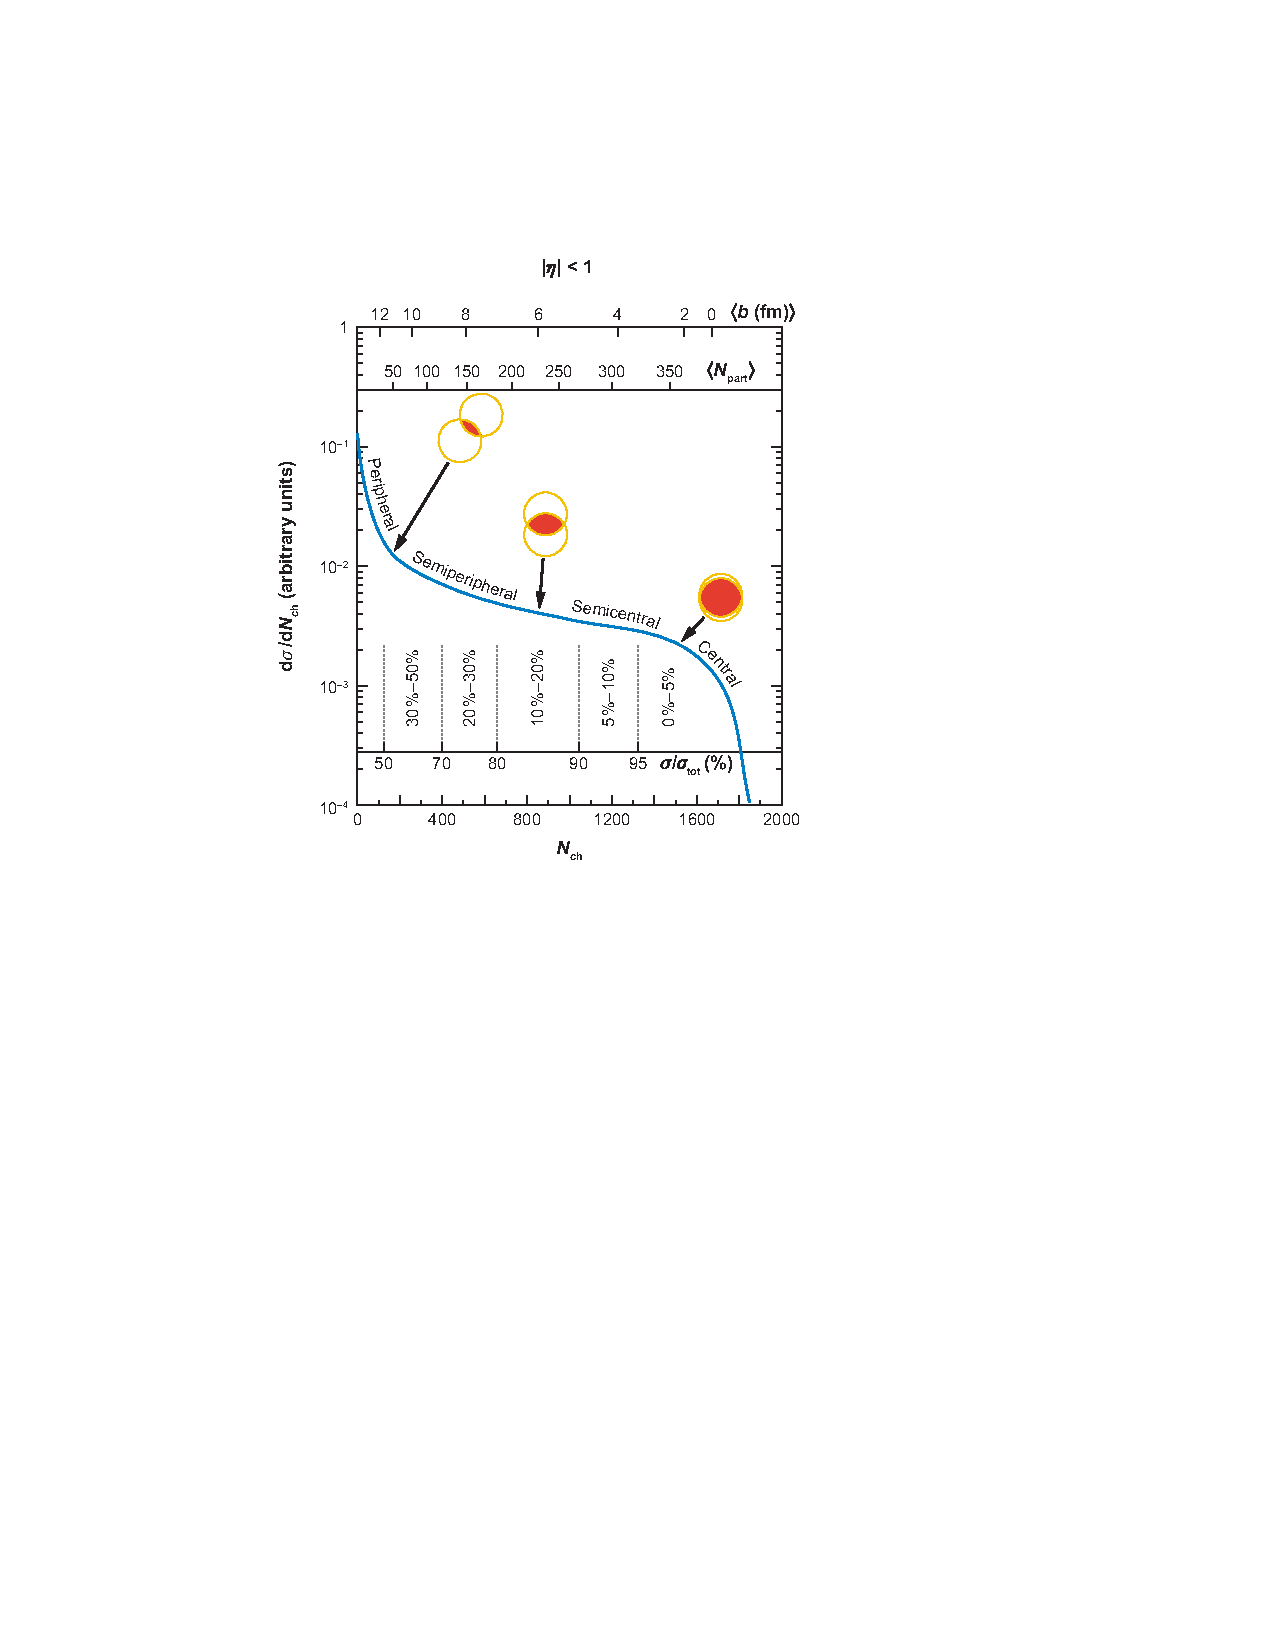
\includegraphics[width=0.45\textwidth]{figures/theory/cent_estimate}
\caption{The correlation between the observable \Nch\ and \Npart\ to determine the centrality distribution. Taken from \cite{doi:10.1146/annurev.nucl.57.090506.123020}. }
\label{fig:cent_estimate}
\end{center}
\end{figure}

%In these collisions, the QGP formed is more lenticular in the transverse direction.
% Of course, the colliding nuclei are not perfectly smooth objects and are made of individual nucleons giving them a non-uniform structure. This results in the energy density in the overlap region being non-uniform with any variations giving rise to pressure gradients that cause azimuthal anisotropies in the momentum distribution of the produced particles. 

%The heavy ion collision system is an extraordinarily useful laboratory to study QCD because it gives access to the otherwise confined partons and provides for a way to study the phase transition between the QGP and ordinary hadronic matter. It is also able to replicate the conditions in the early universe, just after the Big Bang \cite{23, 24}, when it was too hot for hadrons to exist in the form that they do now. 

%We can differentiate different nucleons in the collision as per the following:
%\subparagraph{$\mathrm{N}_{\mathrm{part}}$: } This is the number nucleons that have collided with at least one other nucleon, and can be said to have participated in the heavy ion collision.
%\subparagraph{$\mathrm{N}_{\mathrm{coll}}$: } This is the number of binary collisions that take place between the nucleons of the colliding nuclei. It is typically much larger than \Npart.
%\subparagraph{$\mathrm{N}_{\mathrm{spec}}$: } This is the number nucleons that do not encounter any nucleon from the other nucleus and are just spectators to the collision. 

%The properties of the QGP can be determined by azimuthal correlation measurements \cite{5, 6, 90}, while how it interacts with a high energy parton can be determined by jet studies \cite{91, 92, 69, etc}. 


%%%%%%%%%%%%%%%%%%%%%%%%%%%%%%%%%%%%%%%%%%%%%%%%%%%%%%%%%%%%%%%%%%%%%%%%%




\section{Quark Gluon Plasma}
\label{sec:qgp}
% !TEX root = thesis-ex.tex
The quark-gluon plasma is a state of matter that comprises of free partons and is formed in extreme conditions of temperature and pressure \cite{SHURYAK198071}.
Its study is motivated by the fact that is the only way to access the dynamics of partons that are otherwise confined within hadrons.
Moreover, its thermodynamic properties are of particular interest since it filled the early universe a few microseconds after the Big Bang \cite{PhysRevLett.34.1353}.
The QGP also forms the core of neutron-stars \cite{Linde_1979} and the recent detection of gravitational waves from a neutron-star merger \cite{PhysRevLett.119.161101} has opened new avenues of investigation \cite{Han:2018mtj, PhysRevD.99.023009, PhysRevLett.122.061101}.
These studies have the potential to provide information into the nuclear equation of state since the dynamics of the merger are sensitive to the behavior of extremely dense nuclear matter \cite{PhysRevD.86.063001}.
The increase in temperatures and densities in merging neutron stars allows for probing different regions of the QCD phase diagram.
In particular, differences in gravitational-waves from these systems before and after the merger can be used to provide an observable signature of a first order phase transition \cite{PhysRevLett.122.061102}.
Colliders like RHIC and the LHC on the other hand probe regions that have near zero low baryon densities.
Lattice QCD calculations in these regions show that the transition between a hadronic gas and the QGP occurs at a temperature of approximately 160 MeV and corresponds to an energy density of 0.5 GeV/fm$^3$ \cite{Borsanyi:2010bp}.
This is a smooth crossover that spans a 20--30 MeV temperature range, and can be seen in the QCD phase diagram shown in Figure~\ref{fig:qcd_phase}.
%At lower temperatures and higher values of baryon densities, calculations suggest a presence of a first-order phase transition \cite{PhysRevD.78.074507}.
This phase diagram shows the transition between free quarks and gluons within the QGP and the confined quarks and gluons within hadrons, as a function of temperature $T$ and baryon chemical potential $\mu$.


\begin{figure}[htbp]
\begin{center}
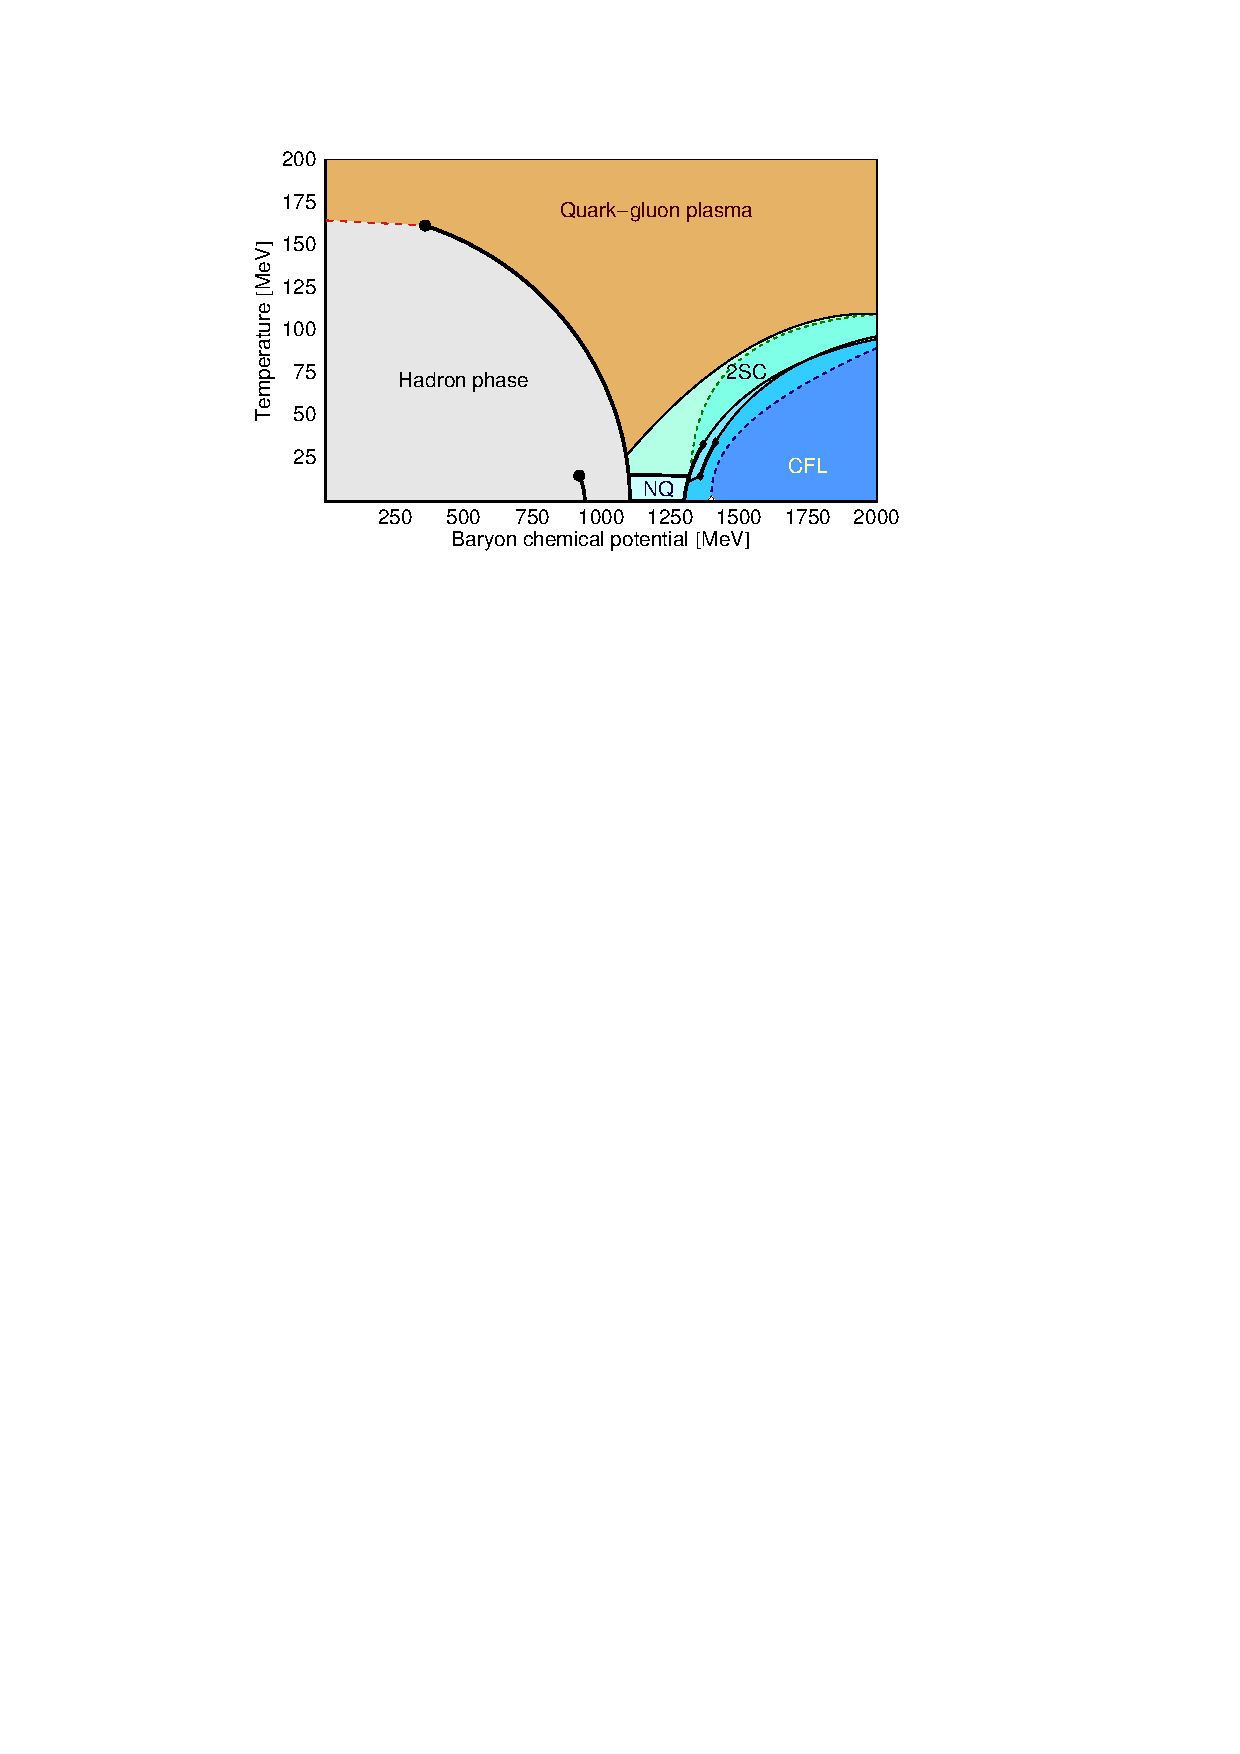
\includegraphics[width=0.45\textwidth]{figures/theory/qcd_phase}
\caption{The QCD phase diagram of nuclear matter as a function of temperature $T$ and baryon chemical potential $\mu$.
The $n\star$ denotes a neutron star.
Figure from from Ref.~\cite{Kronfeld:2012uk}.}
\label{fig:qcd_phase}
\end{center}
\end{figure}

When formed in a heavy ion collision, this state of matter exists for 1-10 fm/c, depending on the collision energy \cite{doi:10.1146/annurev.nucl.46.1.71}.
Hydrodynamic models of photon emission can be used to describe data measured at both RHIC \cite{PhysRevLett.104.132301} and LHC \cite{2016235} energies and suggest that the initial temperature of the QGP is 300--600 MeV \cite{PhysRevC.81.034911}.
As the QGP cools via expansion, its temperature drops below the critical temperature of QCD phase transitions and it forms a hadron gas.
This process, referred to as a chemical freeze-out, occurs at about 160 MeV \cite{Fodor_2004, ADAMS2005102, PhysRevC.93.024917}.
The hadrons formed in this stage continue to interact with each other, but have energies below the threshold for inelastic particle production, resulting mainly in modifications to their momentum spectra.
This continues till the medium cools further and reaches what is called a thermal freeze-out at 100--150 MeV \cite{PhysRevC.69.024904, PhysRevC.72.014908, PhysRevC.75.024910, PhysRevC.88.044910}.

%These measurements paint a picture of the QGP being formed early in the heavy ion collision.It has a non-uniform energy density and temperature determined by the colliding nuclei and collision energy.The QGP then cools and expands as described by relativistic hydrodynamics, and as its temperature falls below 160 MeV, it experiences a crossover phase transition and hadronizes.This system continues to cool and expand, until at 95 GeV there is a thermal freeze-out.

%The QGP can be further characterized by comparing quarkonia production in heavy ion and \pp\ collisions.

%Supposing that the interactions between quarks and gluons are negligible, their energy density can be written in terms of the temperature $T$ and quark chemical potential $\mu$ as:
%
%\begin{align}
%\varepsilon_g &= \frac{16 \pi^2}{30} T^4 \\
%\varepsilon_q+\varepsilon_{\bar{q}} &= 12 \left( \frac{7\pi^2}{120} T^4 + \frac{1}{4}\mu^2 T^2 + \frac{1}{8\pi^2} \mu^4 \right)
%\end{align}
%Then, the thermodynamical quantities of pressure $P$, entropy density $s$ and baryon number density $\rho_B$ are given by:
%
%\begin{align}
%P = \frac{1}{3} \varepsilon, \qquad s = \left(\frac{\partial P}{\partial T}\right)_\mu, \qquad \rho_B = \frac{1}{3} \left( \frac{\partial P}{\partial \mu} \right)_T
%\end{align}
%
%Using the framework of the MIT Bag Model and assuming the QGP as an ideal gas with a bag constant $\mathcal{B}$ that parameterizes the vacuum pressure \cite{Muller1993, Yagi:2005yb}, the equation of state of the QGP can be written as
%
%\begin{align}
%\varepsilon &= \varepsilon_g(T, \mu) + \varepsilon_q(T, \mu) + \varepsilon_{\qbar} (T, \mu) + \mathcal{B} \\
%P &= P_g(T, \mu) + P_q(T, \mu) + P_{\qbar} (T, \mu) - \mathcal{B}
%\end{align}
%
%This model considers quarks and gluons to move freely inside a ``bag'' and postulates that a deconfined medium can be formed by compressing the bags together.Assuming a baryon free case with $\mu = 0$ and idealizing hadronic matter as a gas of non-interacting massless pions:
%
%\begin{align}
%\varepsilon_\pi = \frac{3\pi^2}{30} T^4, \qquad P_\pi = \frac{1}{3} \varepsilon_\pi
%\end{align}
%%%%%%%%%%%%%%%%%%%%%%%%%%%%

The QGP was initially thought to be a weakly coupled parton gas because of asymptotic freedom from QCD.
The highly energetic collisions such as those at the LHC would imply weak interactions between the partons that make up the plasma \cite{PhysRevLett.34.1353, heinz2013collective, 10.1007/978-1-4020-2705-5_14}.
This would result in rare scatterings between the constituents of the gas, washing out any spatial anisotropies based on ``'lumpy''-ness of the colliding nuclei or the collision geometry.
On the other hand, a strong coupling within the QGP would result in the pressure gradients in the medium being driven by hydrodynamics and spatial anisotropies would be transformed to momentum anisotropies in the particles produced as shown in Figure~\ref{fig:overlap} \cite{Busza:2018rrf}.
In this picture, the non-uniform structure of the colliding nuclei would cause a momentum anisotropy \cite{Ster:1999ib} that would be further enhanced when looking at collisions that are less central and do not have perfect overlap between the colliding nuclei \cite{Poskanzer:1999ea, Pinkenburg:1999ya}.
These observations were seen in azimuthal correlation measurements implying that the medium is indeed strongly coupled \cite{Aaboud:2018ves, PhysRevLett.91.182301, Sirunyan:2017fts, PhysRevLett.116.132302}.

\begin{figure}[htbp]
\begin{center}
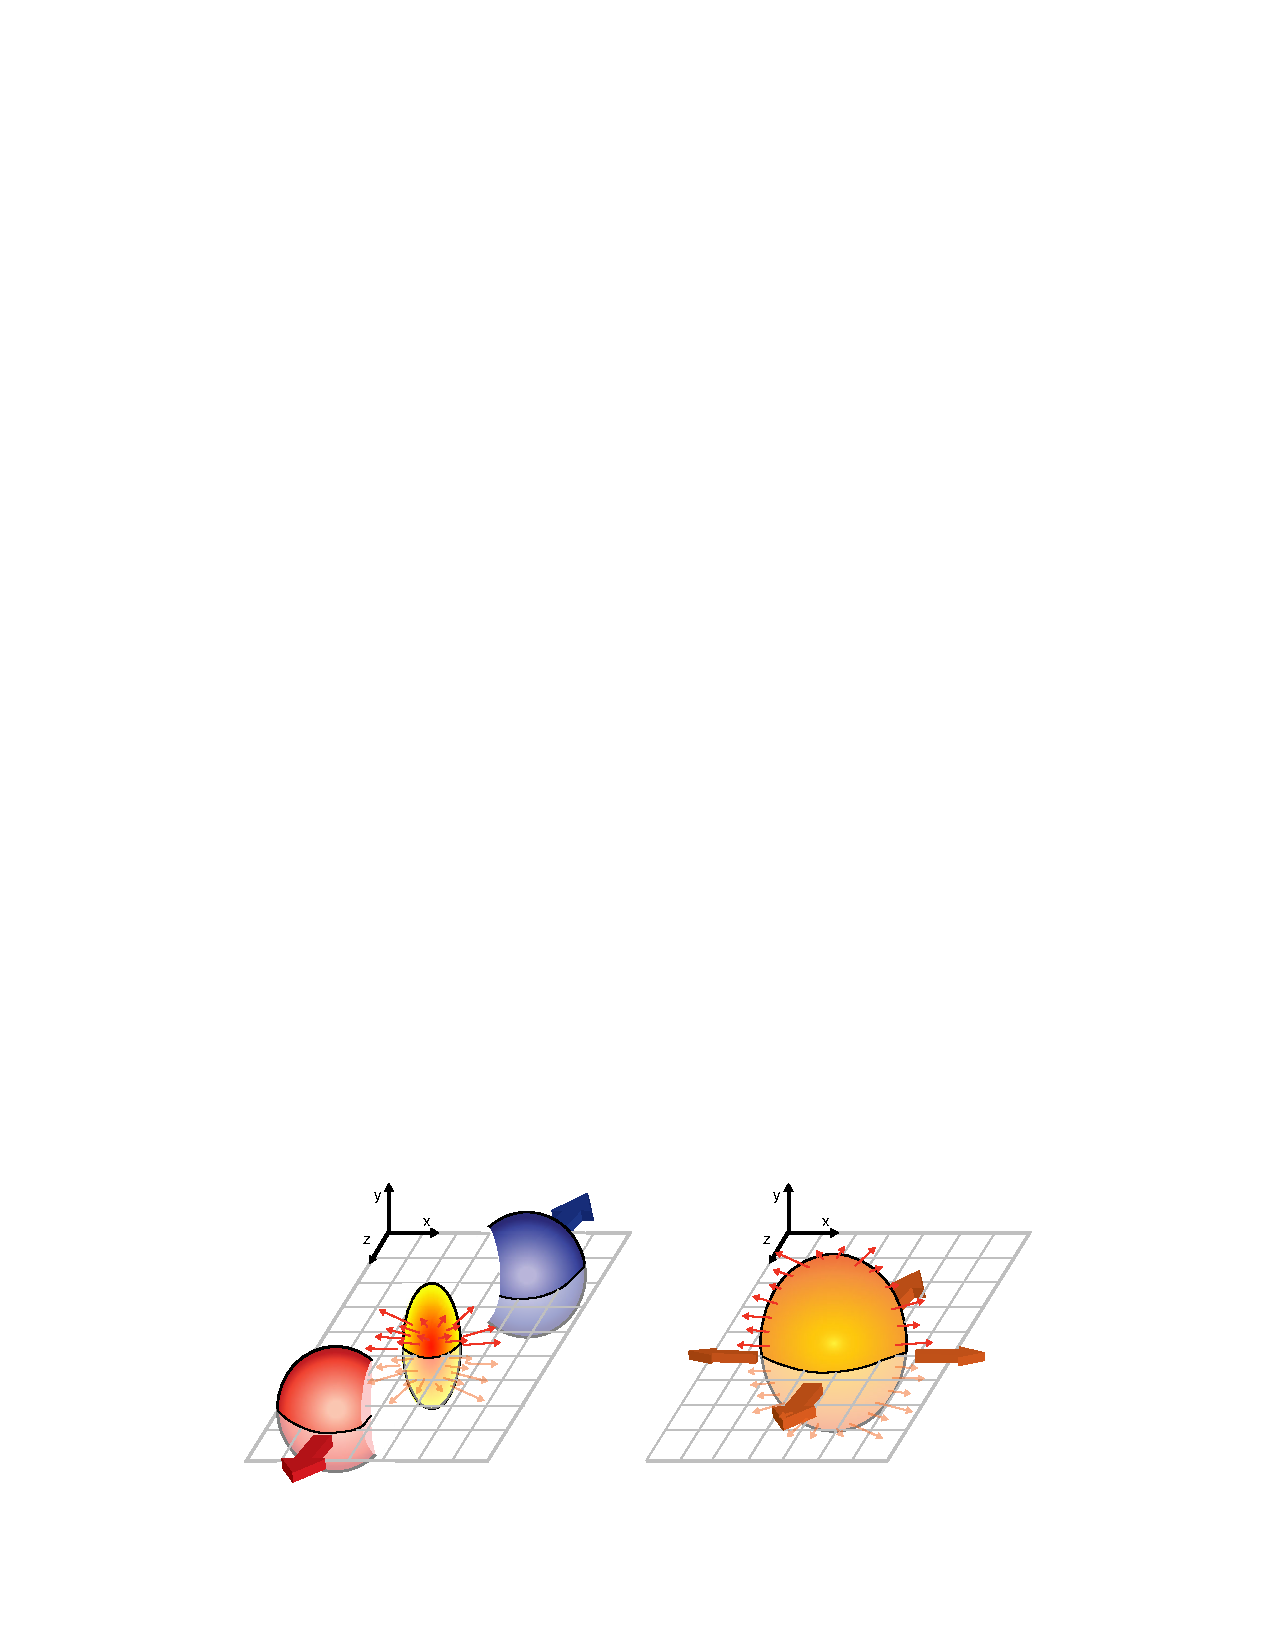
\includegraphics[width=0.85\textwidth]{figures/theory/overlap}
\caption{Schematic diagrams of the initial overlap region (left) and the final spatial anisotropy generated (right).
Taken from Ref.~\cite{RevModPhys.90.025005}.}
\label{fig:overlap}
\end{center}
\end{figure}


%At the peak energy density of the collision, the system cannot be described at the level of hadrons, and has to be described in terms of quarks and gluons.The initial anisotropic energy density being reflected in the azimuthal variation of particle production implies a strongly coupled medium that expands hydrodynamically, with a faster expansion in the direction of larger gradients and hence resulting a momentum anisotropy.
%A Fourier Transform of the angular distribution of charged hadrons in the collision debris can quantify these momentum anisotropies and give the anisotropic flow coefficients $v_n$, defined as :

The azimuthal angular distribution of particles produced in a heavy ion collision can be expanded in a Fourier series as \cite{Poskanzer:1998yz}: 

\begin{align}
\frac{d\bar{N}}{d\phi} = \frac{N}{2\pi} \left( 1 + 2 \sum_{n=1}^{\infty} v_{n} \cos(n(\phi-\Psi_n)) \right).
\end{align}
where  $N$ is the particle yield, $\phi$ is the azimuthal angle in the transverse plane and $\Psi_n$ is the orientation of the $n^{\mathrm{th}}$ order symmetry plane and is called the reaction plane.
The reaction plane, along with the participant plane, are shown in Figure~\ref{fig:reaction_plane}.
The coefficient $v_n = \langle \cos[n(\phi_i - \Psi_n)] \rangle$ is the magnitude of the $n^{\rm{th}}$ order azimuthal anisotropy, and is referred to as the flow harmonic.
The first harmonic $v_1$ is called directed flow because it indicates a particular direction, while the second harmonic $v_2$ is called elliptic flow since the azimuthal distribution in polar coordinates for $v_2 \neq 0$ is an ellipse.
These are shown in Figure~\ref{fig:flow_v1_v2} \cite{Voloshin:2008dg}.
The azimuthal correlations that are a result of flow can be described by relativistic hydrodynamics \cite{Teaney:2001av, HIRANO2006299}.
A comparison of anisotropies measured in terms of $v_n$ in Ref.~\cite{ALICE:2011ab} and a hydrodynamic model described in Ref.~\cite{Niemi:2015qia} is shown in Figure~\ref{fig:flow_coeff}.


\begin{figure}
\begin{center}
  \begin{minipage}[b]{0.4\textwidth}
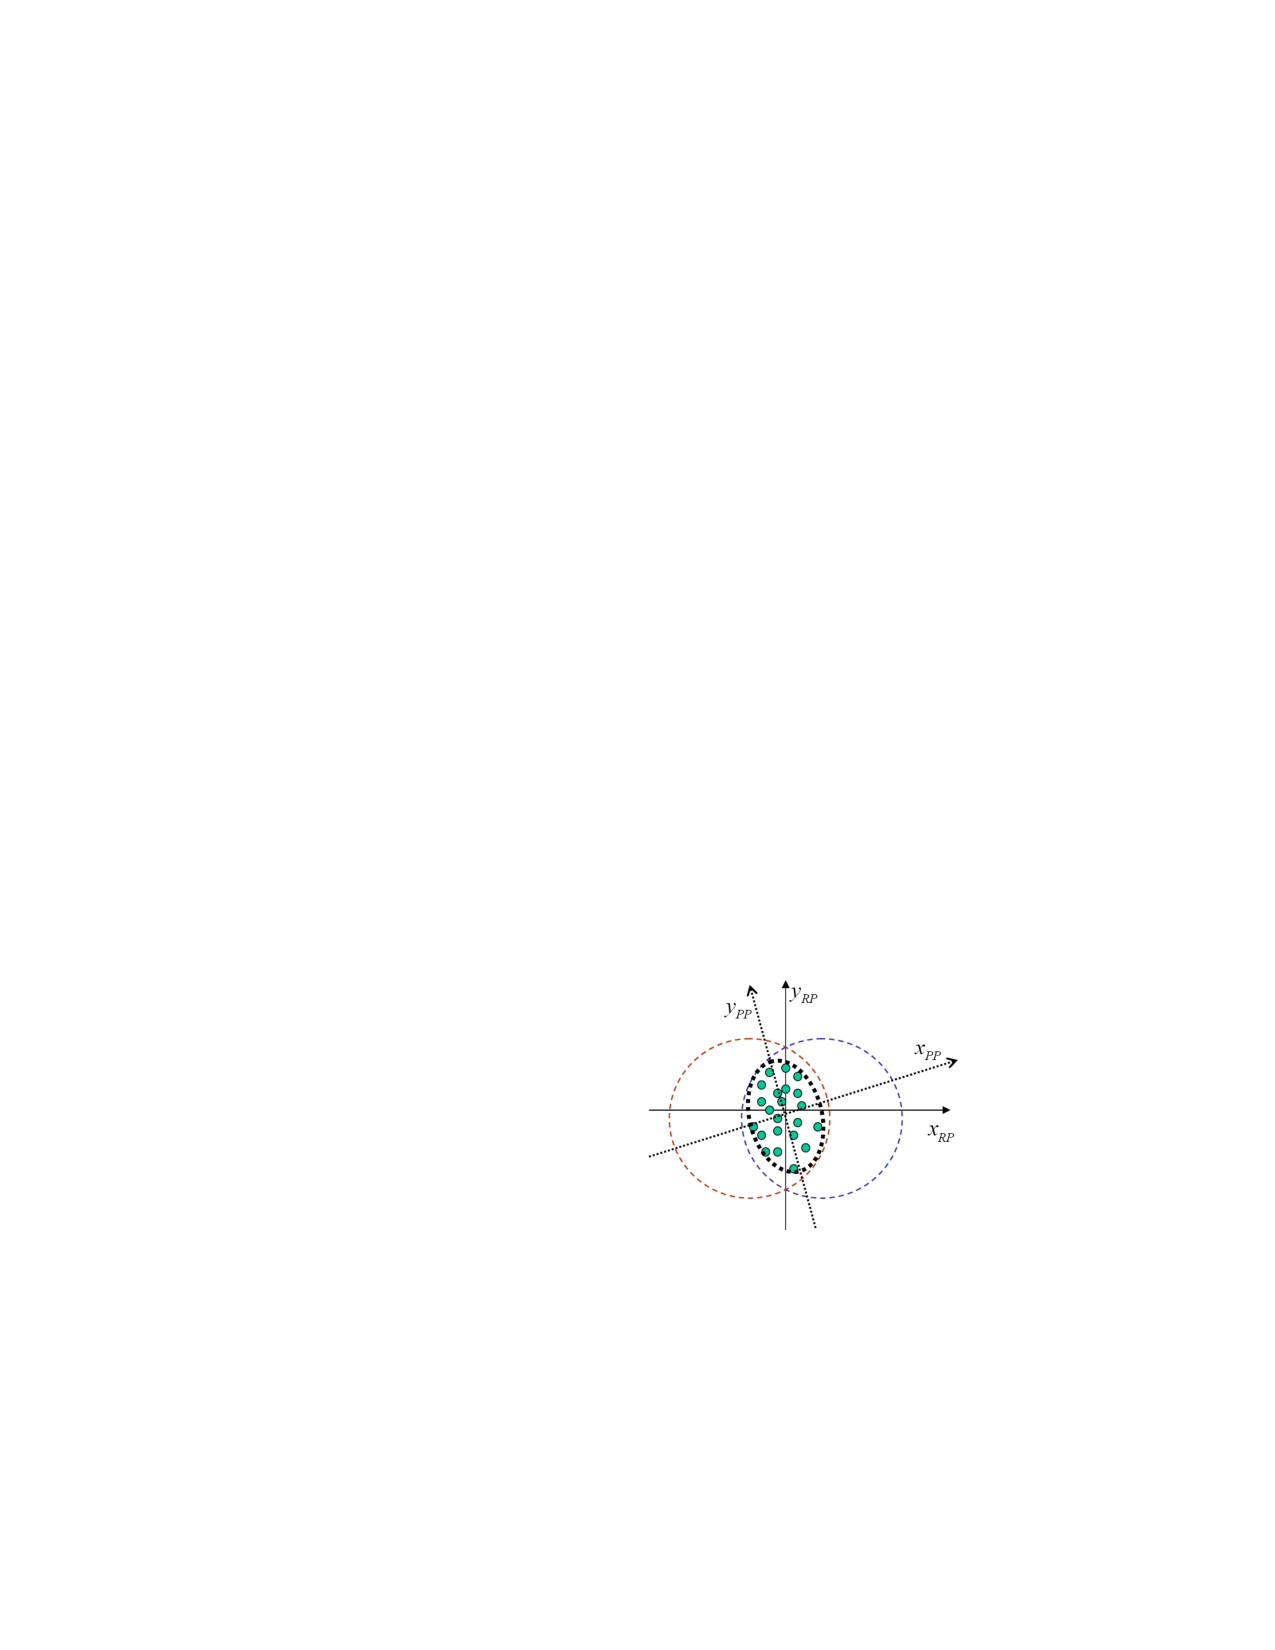
\includegraphics[width=\textwidth]{figures/theory/reaction_plane}
\caption{Definitions of the Reaction and Participant Plan coordinate systems.
Figure taken from Ref.~\cite{Voloshin:2008dg}.}
\label{fig:reaction_plane}
  \end{minipage}
 \qquad  \qquad  \qquad
  \begin{minipage}[b]{0.4\textwidth}
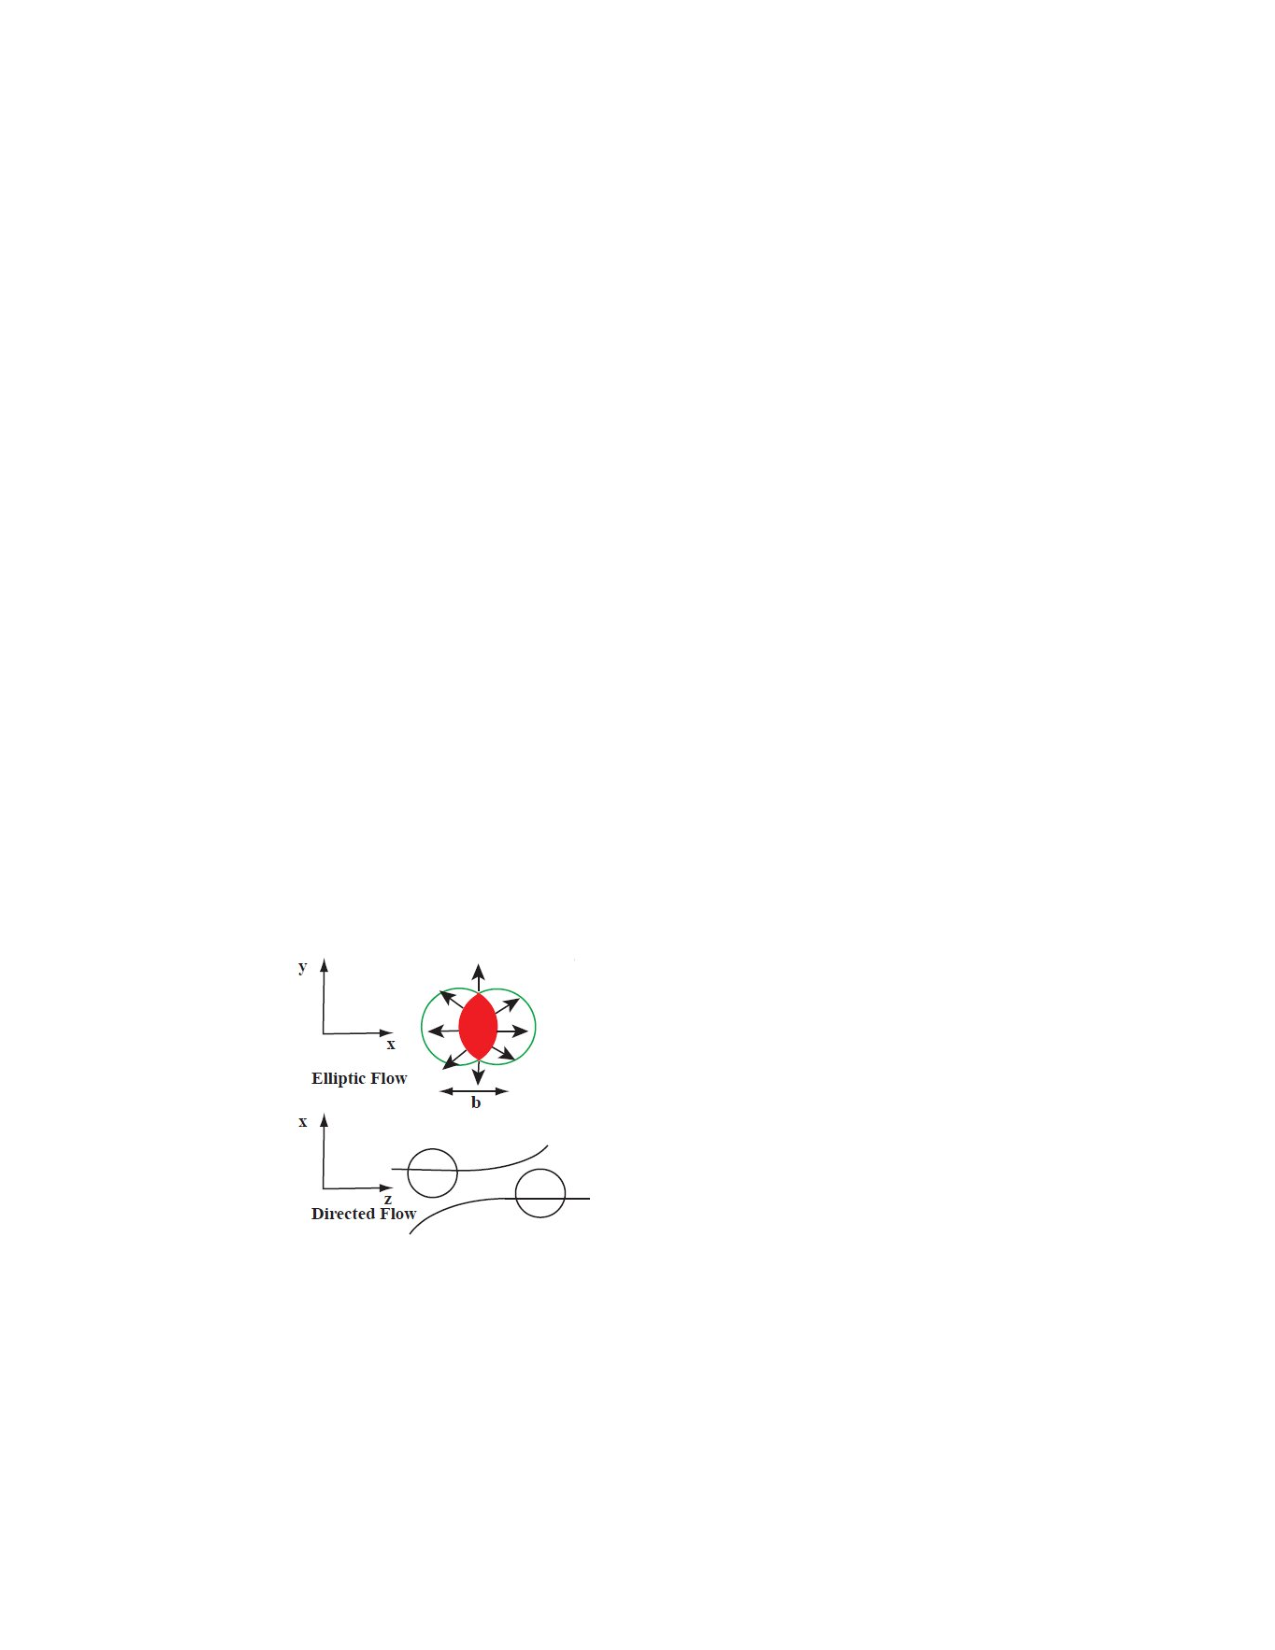
\includegraphics[width=\textwidth]{figures/theory/flow_v1_v2}
\caption{Schematics of elliptic and directed flow.
Figure taken from Ref.~\cite{Voloshin:2008dg}.}
\label{fig:flow_v1_v2}
  \end{minipage}
  \end{center}
\end{figure}

\begin{figure}[htbp]
\begin{center}
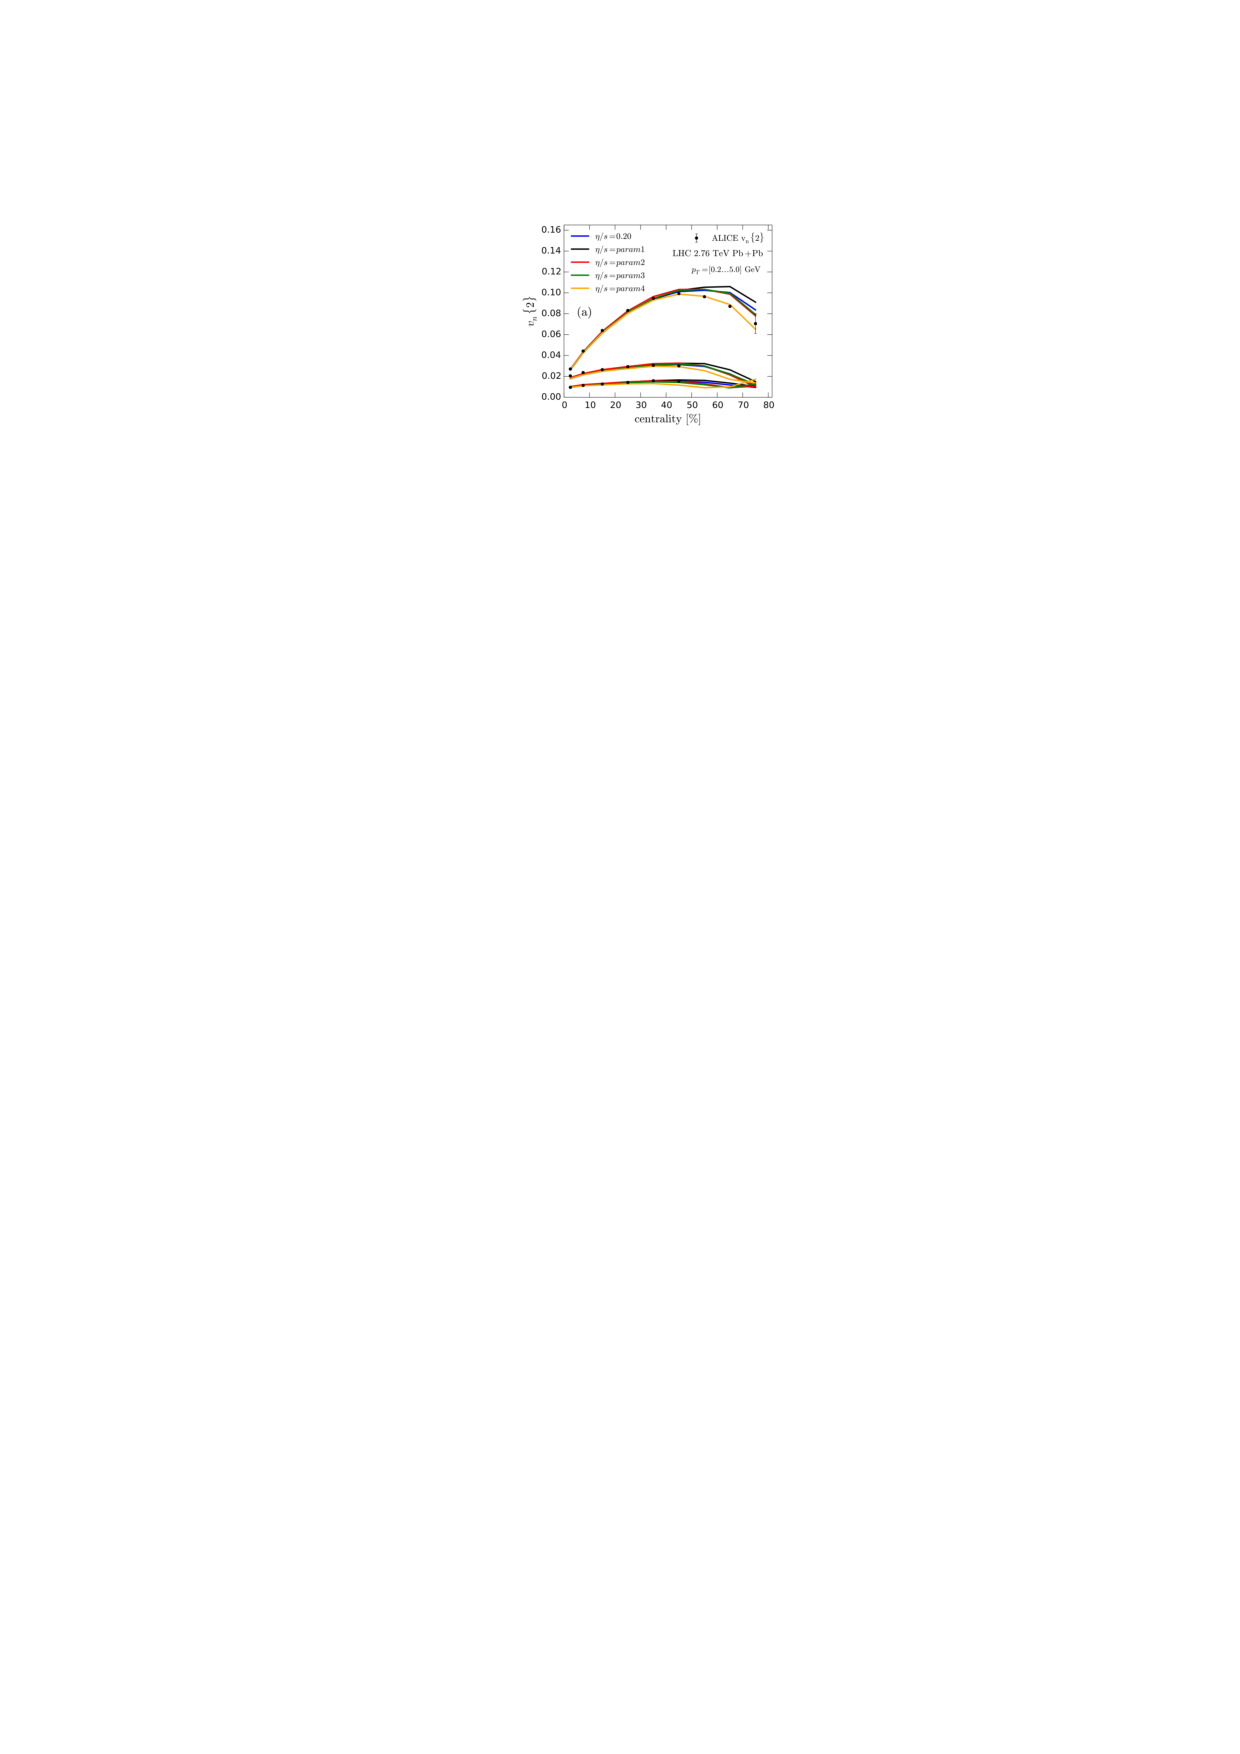
\includegraphics[width=0.45\textwidth]{figures/theory/flow_coefficients}
\caption{Comparison of a hydrodynamic model from Ref.~\cite{Niemi:2015qia} to anisotropy measurements by ALICE \cite{ALICE:2011ab} for different parameterizations of $\eta / s $ and for different $v_n$, {\it{n}} = 2, 3, 4 from top to bottom, as a function of collision centrality.
Figure taken from Ref.~\cite{Busza:2018rrf}.}
\label{fig:flow_coeff}
\end{center}
\end{figure}

The measured anisotropies can be used to constrain the specific viscosity given by the ratio of viscosity to entropy density, $\eta / s$, and have shown that the QGP is a near perfect liquid with an $\eta / s$ of near the theoretical minimum of $1/4\pi$ \cite{ARSENE20051, GYULASSY200530}.
In fact, this low shear viscosity is what allows the initial fluctuations in the energy density to survive the chemical freeze-out.



























\section{Jets and Jet Quenching}
\label{sec:jets}
% !TEX root = thesis-ex.tex


Hard scatterings in particle collisions result in the production of highly energetic partons that form conical sprays of hadrons called jets. A schematic of this process is shown in Figure~\ref{fig:feynman_jet}. Jet production in a vacuum is well described in context of perturbative QCD \cite{Sjostrand:2007gs} where processes involving large momentum transfers like high \pt\ hadron production can be described in terms of the parton distribution functions, scattering cross sections, and final state fragmentation functions as shown below \cite{Qin:2015srf}:


\begin{figure}[htbp]
\begin{center}
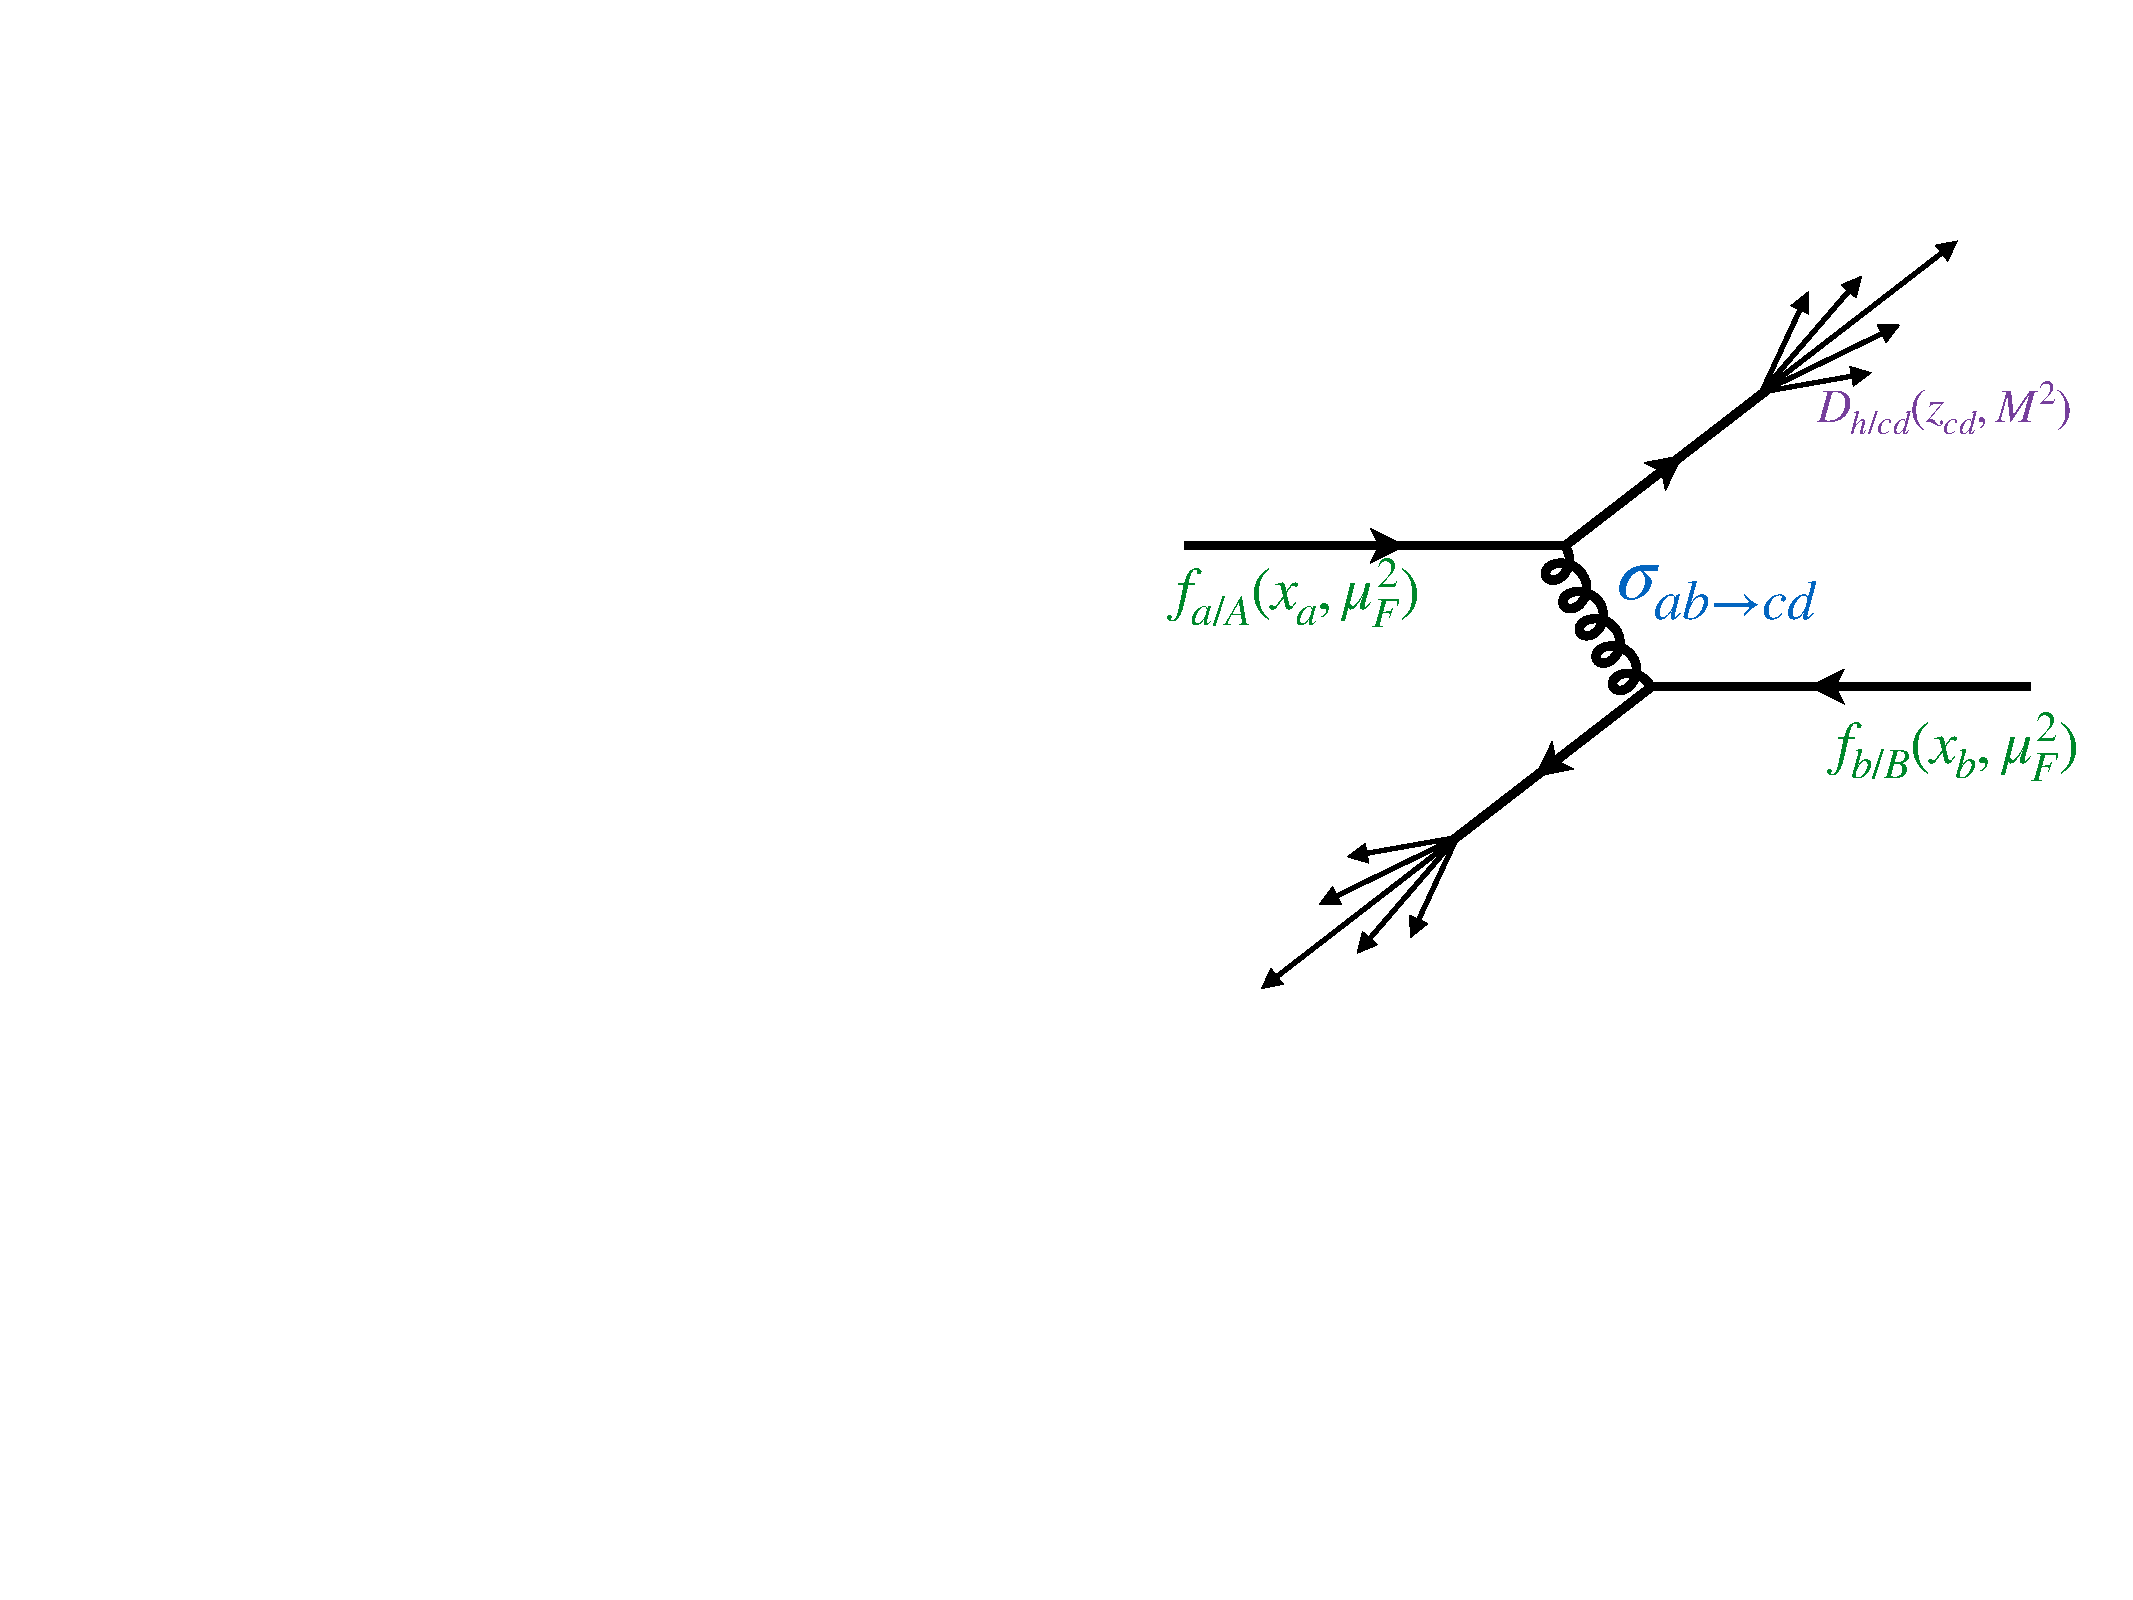
\includegraphics[width=0.35\textwidth]{figures/theory/feynman_jet}
\caption{Jet production from the process $pp \rightarrow hX$, factorizing in terms of the parton distribution functions, scattering cross sections, and jet fragmentation functions. \cite{Qin:2015srf}}
\label{fig:feynman_jet}
\end{center}
\end{figure}



\begin{align}
\label{eq:hadronCS}
d \sigma_{pp \rightarrow hX} \approx & \sum_{abjd} \int dx_a \int dx_b \int dz_j f_{a/p} (x_a, \mu_f) \otimes f_{b/p} (x_b, \mu_f) \\
& \otimes d\sigma_{ab\rightarrow jd} (\mu_f, \mu_F, \mu_R)  \nonumber \\
& \otimes D_{j \rightarrow h} (z_j, \mu_f) \nonumber
\end{align}
where $x_a = p_a/P_A, x_b = p_b / P_b$ are the initial momentum fractions carried by the interacting partons, $z_j = p_h / p_j$ is the momentum fraction carried by the final observed hadron. $f_{a/p} (x_a, \mu_f)$ and $f_{b/p} (x_b, \mu_f)$ are the two parton distribution functions (PDFs), $d\sigma_{ab\rightarrow jd} (\mu_f, \mu_F, \mu_R)$ is the differential cross section for parton scattering and $D_{j\rightarrow }(z_j,\mu_F)$ is the fragmentation function (FFs) for parton $j$ to hadron $h$. $\mu_f$ and $\mu_F$ are the factorization scales and $\mu_R$ is the renormalization scale, and are typically taken to be the same hard scale $Q$. The PDFs characterize the initial state and represent the probability of finding a parton with momentum fraction $x$ (shown in Figure~\ref{fig:bjorkenX}) in the initial hadron, while the FFs describe the probability of fragmenting to a hadron $h$ with given kinematic properties.

\begin{figure}[htbp]
\begin{center}
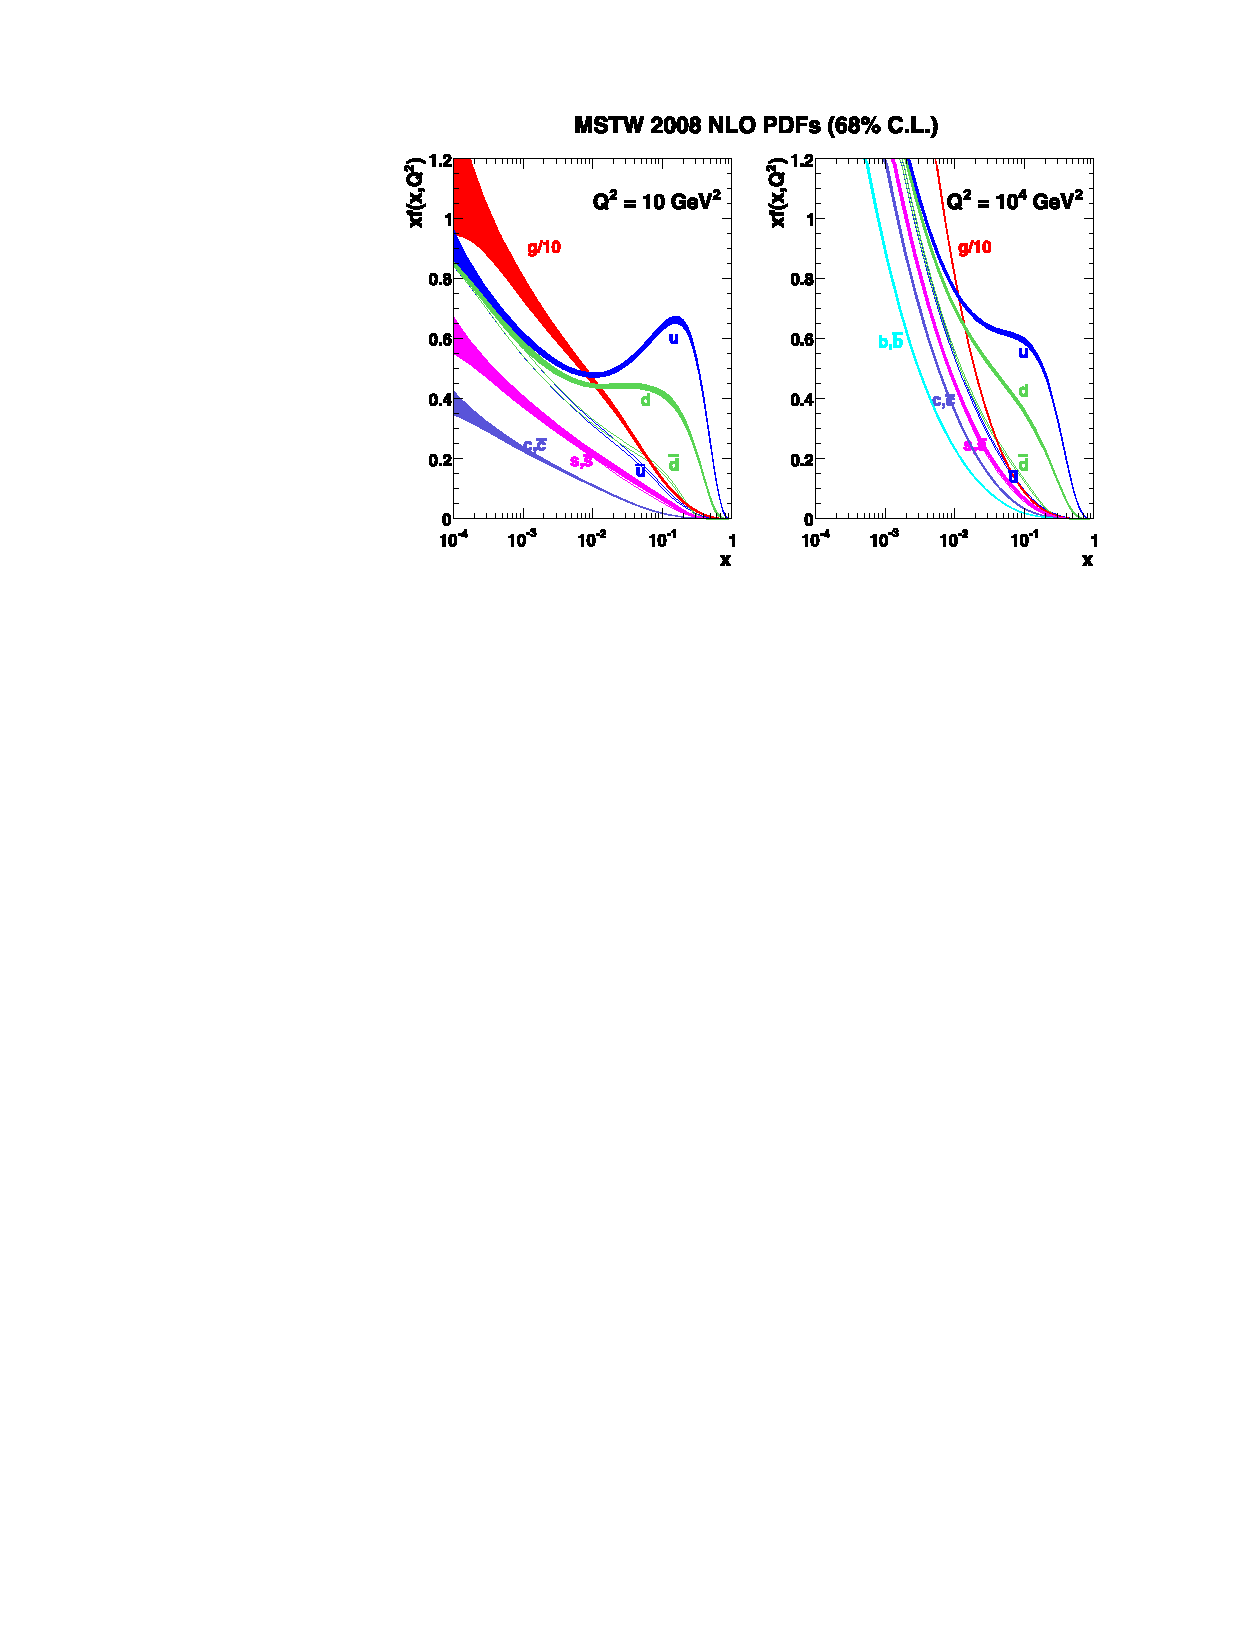
\includegraphics[width=0.55\textwidth]{figures/theory/bjorkenX}
\caption{The next to leading order (NLO) PDFs at (left) $Q^2 = 10 \mathrm{GeV}^2$ and (right) $Q^2 = 10^4 \mathrm{GeV}^2$. The band is the associated one-sigma (68\%) confidence level uncertainty. Taken from \cite{Martin2009}}
\label{fig:bjorkenX}
\end{center}
\end{figure}


%Both the PDFs and FFs are universal and their scale dependence evolves via the Dokshitzer-Gribov-Lipatov-Altarelli-Parisi (DGLAP) equations \cite{ALTARELLI1977298, Gribov:1972ri, Dokshitzer:1977sg}. These calculations can be compared to the inclusive charged particle distributions in \sqrts = 13 TeV \pp\ collisions and shown in Figure~\ref{fig:inclhadronCS}.  



%The energy lost by a jet serves as further confirmation that the medium produced in a heavy ion collision is strongly coupled.

In the case of heavy ion collisions, the jet observables can be modified due to two sources: the nuclear PDF being distinct from a proton PDF, and the formation of the quark gluon plasma.

The former is collectively referred to as cold nuclear matter (CNM) effect, and can be quantified by defining a nuclear modification factor for the PDF:

\begin{align}
R_a^A (x, Q^2) = \frac{f_{a/A} (x, Q^2)}{f_{a/p}(x, Q^2)}
\end{align}
where $f_{a/A}$ and $f_{a/p}$ are the nuclear and proton PDFs respectively. This $R_a^A$ factor is determined by global fits to data from DIS measurements \cite{PhysRevC.76.065207, PhysRevD.69.074028, Eskola_2009}. CNM effects include the following contributions:
\begin{itemize}
\item Shadowing: This is a destructive interference effect that reduces the interactions of a nucleon incident on a nucleus within its interior and on its back face. This effect reduces the effective number of nucleons in an inelastic interaction to $A^{2/3}$. For $Q^2$ of the order of a few $\mathrm{GeV}^2$, this effect dominates for $x < 0.05$ and implies $R_a^A (x, Q^2) < 1$  \cite{PhysRevLett.64.1342}.
\item Anti-shadowing: This compensates for the shadowing effect based on the momentum sum rule, and for $Q^2$ of the order of a few $\mathrm{GeV}^2$ implies $R_a^A (x, Q^2) > 1$ over the region $0.05 < x < 0.20$.
\item EMC: The modification of the nuclear structure function was first observed by the European Muon Collaboration \cite{AUBERT1983275}. Recent observations have suggested that the effect is caused by short-range correlated nucleon pairs within nuclei \cite{PhysRevC.85.047301}. For $Q^2$ of the order of a few $\mathrm{GeV}^2$, this effect dominates for $0.2 < x < 0.80$ and implies $R_a^A (x, Q^2) < 1$.
\item  Fermi Motion: This effect considers the motion of the nucleons within the nucleus. It results in $R_a^A (x, Q^2) > 1$  over the $x > 0.8$ region for $Q^2$ of the order of a few $\mathrm{GeV}^2$ \cite{Saito:1985ct}.
\end{itemize}

Cold nuclear matter effects are experimentally measured using $p+A$ systems where the size and shape of the plasma, and hence any effects thereof, are a lot smaller. 

The second source of modification is the formation of the hot and dense quark gluon plasma. The hot nuclear matter effects further serve as an independent confirmation that the medium formed is strongly interacting. Jets are formed early enough that they traverse the Quark Gluon Plasma and as strongly interacting particles, are both affected by, and affect the QGP. This interaction typically results in the jet losing energy and forward momentum \cite{2012176, ATLAS:2017wvp}, with the lost energy being deposited in the medium \cite{Khachatryan2016}. Jets can also pick up momentum transverse to the parton direction \cite{Chatrchyan:2012nia}. The hot nuclear matter effects can be considered to be a combination of collisional and radiative energy losses summarized in Figure~\ref{fig:jetEnergyLoss}.

\begin{figure}[htbp]
\begin{center}
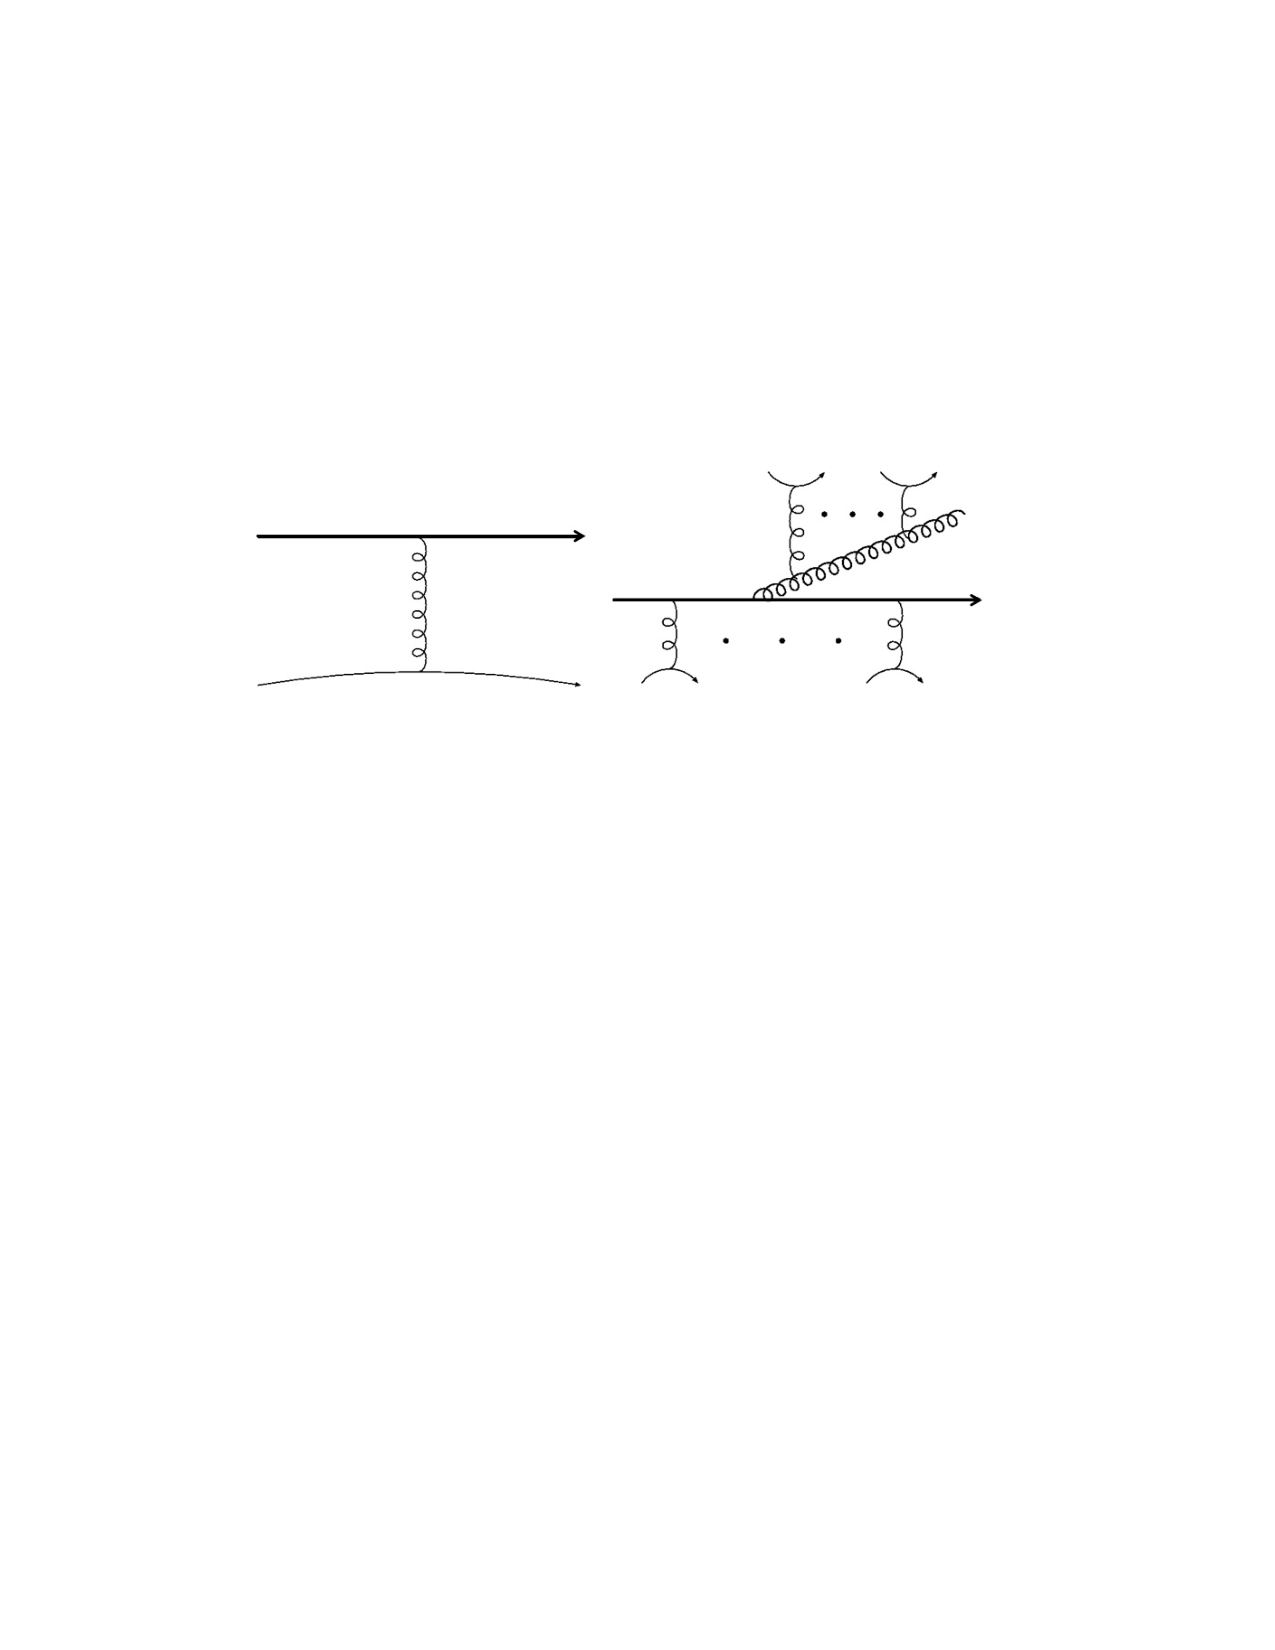
\includegraphics[width=0.75\textwidth]{figures/theory/jetEnergyLoss}
\caption{The typical diagrams for (left) collisional and (right) radiative energy losses for a parton in a hard scattering as it propagates through the QGP. Taken from \cite{Qin:2015srf}}
\label{fig:jetEnergyLoss}
\end{center}
\end{figure}

\begin{itemize}
\item Collisional energy loss: This is a combination of elastic and inelastic collisions of the hard parton with the constituents of the quark gluon plasma. 
\item Radiative energy loss: This is the larger source of parton energy loss and jet quenching. These are modified by the presence of the plasma due to scatterings off of the plasma constituents. A variety of radiative energy loss frameworks that have been developed include: Baier-Dokshitzer-Mueller-Peigne-Schiff-Zakharov (BDMPS-Z) \cite{BAIER1997291}, Gyulassy, Levai and Vitev (GLV) \cite{Gyulassy:1999zd}, Amesto-Salgado-Wiedemann (ASW) \cite{Wiedemann:2000za},  Arnold-Moore-Yaffe (AMY) \cite{Arnold:2001ba} and higher twist (HT) \cite{Guo:2000nz}.
\end{itemize}

\subparagraph{Collisional energy loss} This is a combination of elastic and inelastic collisions of the hard parton with the constituents of the quark gluon plasma. The 

Both hot and cold nuclear matter effects can be described by modifying Equation~\ref{eq:hadronCS} as:
\begin{align}
d \sigma_{AB \rightarrow hX}  \approx & \sum_{abjj'd} f_{a/A} (x_a) \otimes f_{b/B} (x_b) \\ 
& \otimes d\sigma_{ab\rightarrow jd} (\mu_f, \mu_F, \mu_R)  \nonumber \\
& \otimes P_{j\rightarrow j'} \nonumber \\
& \otimes D_{h \rightarrow j'} (z_j, \mu_f) \nonumber 
\end{align}

where the additional $P_{j\rightarrow j'}$ describes the interaction of the hard parton with the colored medium. This is typically taken as part of the fragmentation modification as:

\begin{align}
\widetilde{D}_{h \rightarrow j'} (z_j, \mu_f) \approx \sum_{j'} P_{j\rightarrow j'} (p_{j'} | p_j) \otimes D_{h\rightarrow j'} (_{j'})
\end{align}


\subsection{Jet Reconstruction}
Jets can reconstructed by clustering algorithms that take in a variety of inputs. The algorithm used in ATLAS is the \antikt\ clustering algorithm \cite{Cacciari:2008gp}. This algorithm clusters soft particles around hard ones in the following manner:

\begin{itemize}
\item Calculate all distances $d_{ij}$ between entities $i$ and $j$, and distance $d_{iB}$ between entity $i$ and beam $B$.
\item Identify the smallest distances such that for the smallest distance $d_{ij}$, the entities $i$ and $j$ are combined and return to beginning.
\item If the smallest distance is $d_{iB}$, then take $i$ as the jet and remove it from the list of entities and return to beginning.
\item Continue the procedure till the list of items is empty.
\end{itemize}

In general the distance $d_{ij}$ between the objects is found the via the prescription

\begin{align}
d_{ij} &= \mathrm{min} (k_{Ti}^{2p} , k_{Tj}^{2p}) \frac{\Delta_{ij}^2}{R^2}  \\
d_{iB} &= k_{Ti}^{2p}
\end{align}

where $k_{Ti}$ is the transverse momentum of particle $i$ and $\Delta_{ij} = \sqrt{\Delta\eta_{ij}^2 + \Delta\phi_{ij}^2}$ is the distance between particles $i$ and $j$ in $\eta-\phi$ space. $R$ the distance parameter and reflects the size of the jet being considered. In the case of the \antikt\ algorithm, $p = -1$. Other popular clustering algorithms like \kt\ \cite{Catani:1993hr} and Cambridge/Aachen \cite{Dokshitzer:1997in} use $p = 1$ and $p=0$ respectively. The behavior of the different clustering algorithms is shown in Figure~\ref{fig:JetClustering}. 

\begin{figure}[htp]
\centering
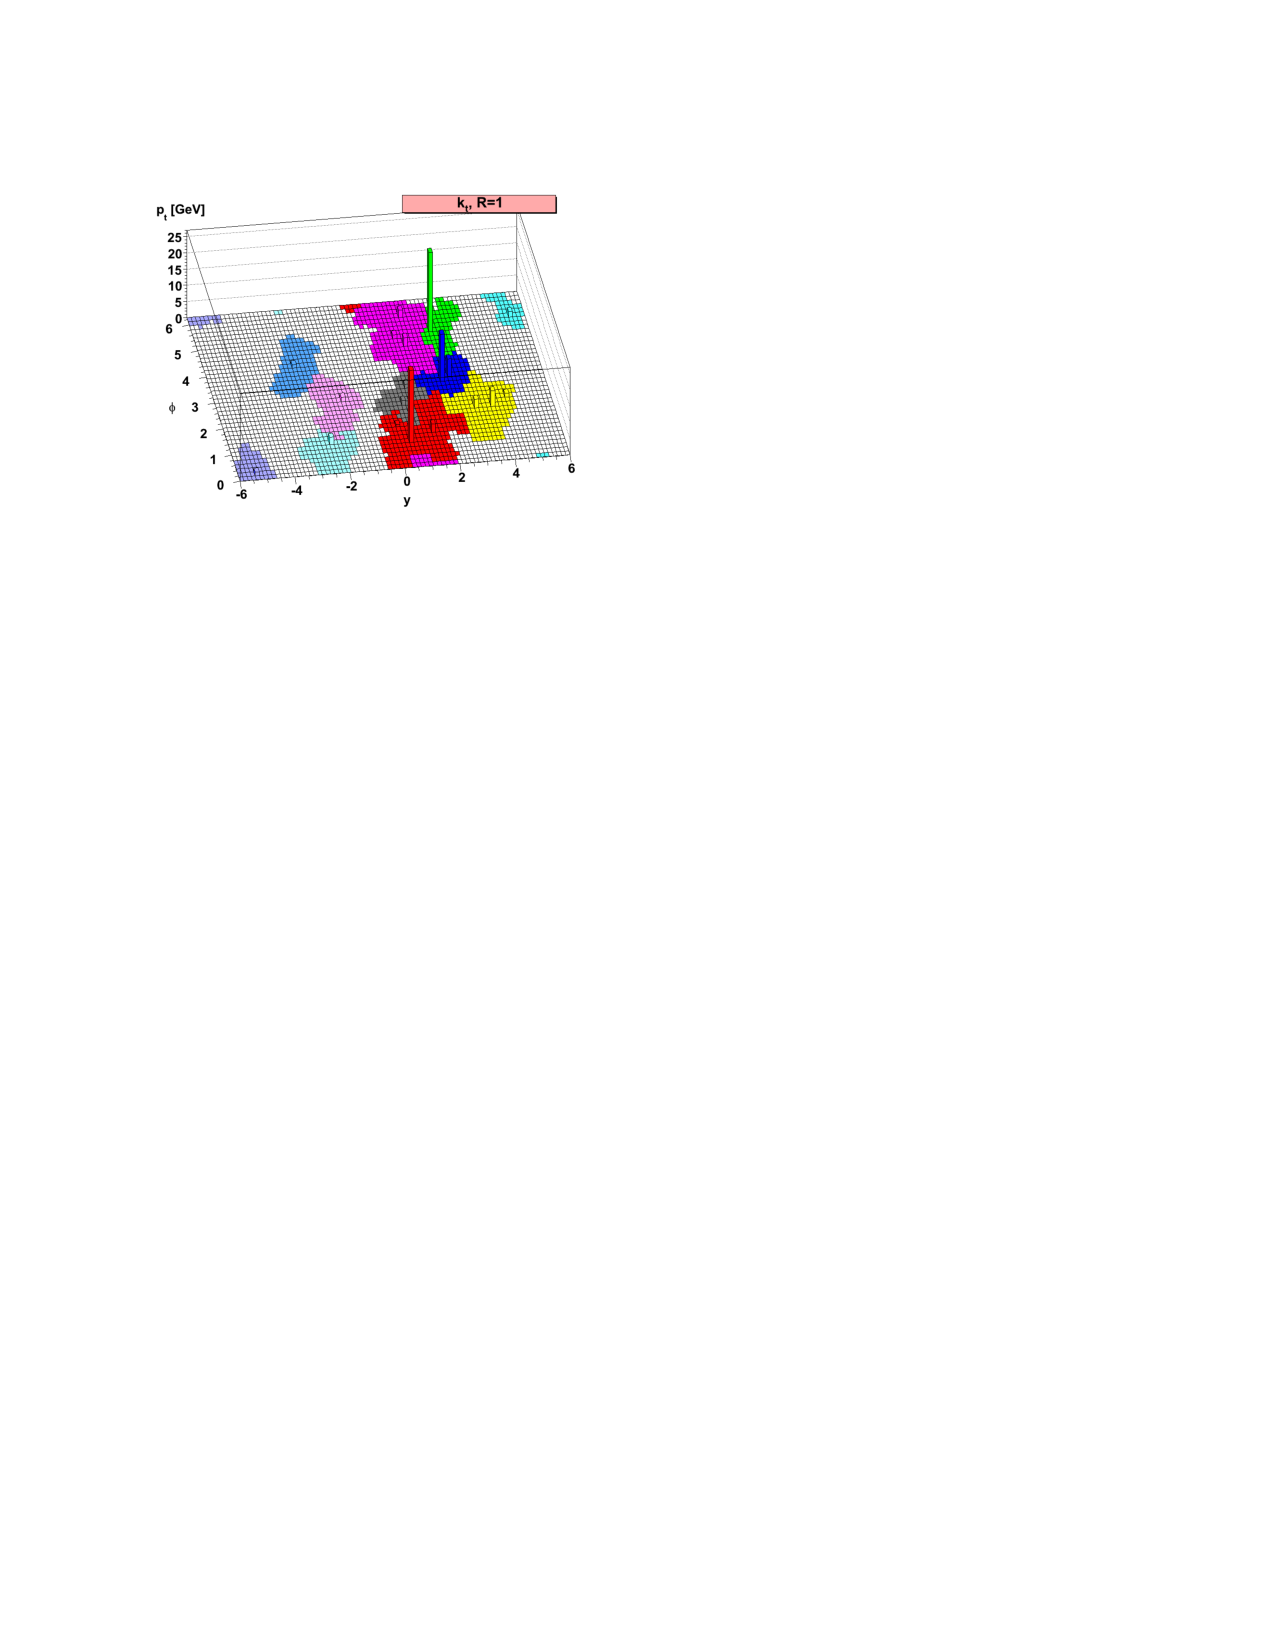
\includegraphics[width=.3\textwidth]{jetMeasurements/jetReco_kt}\hfill
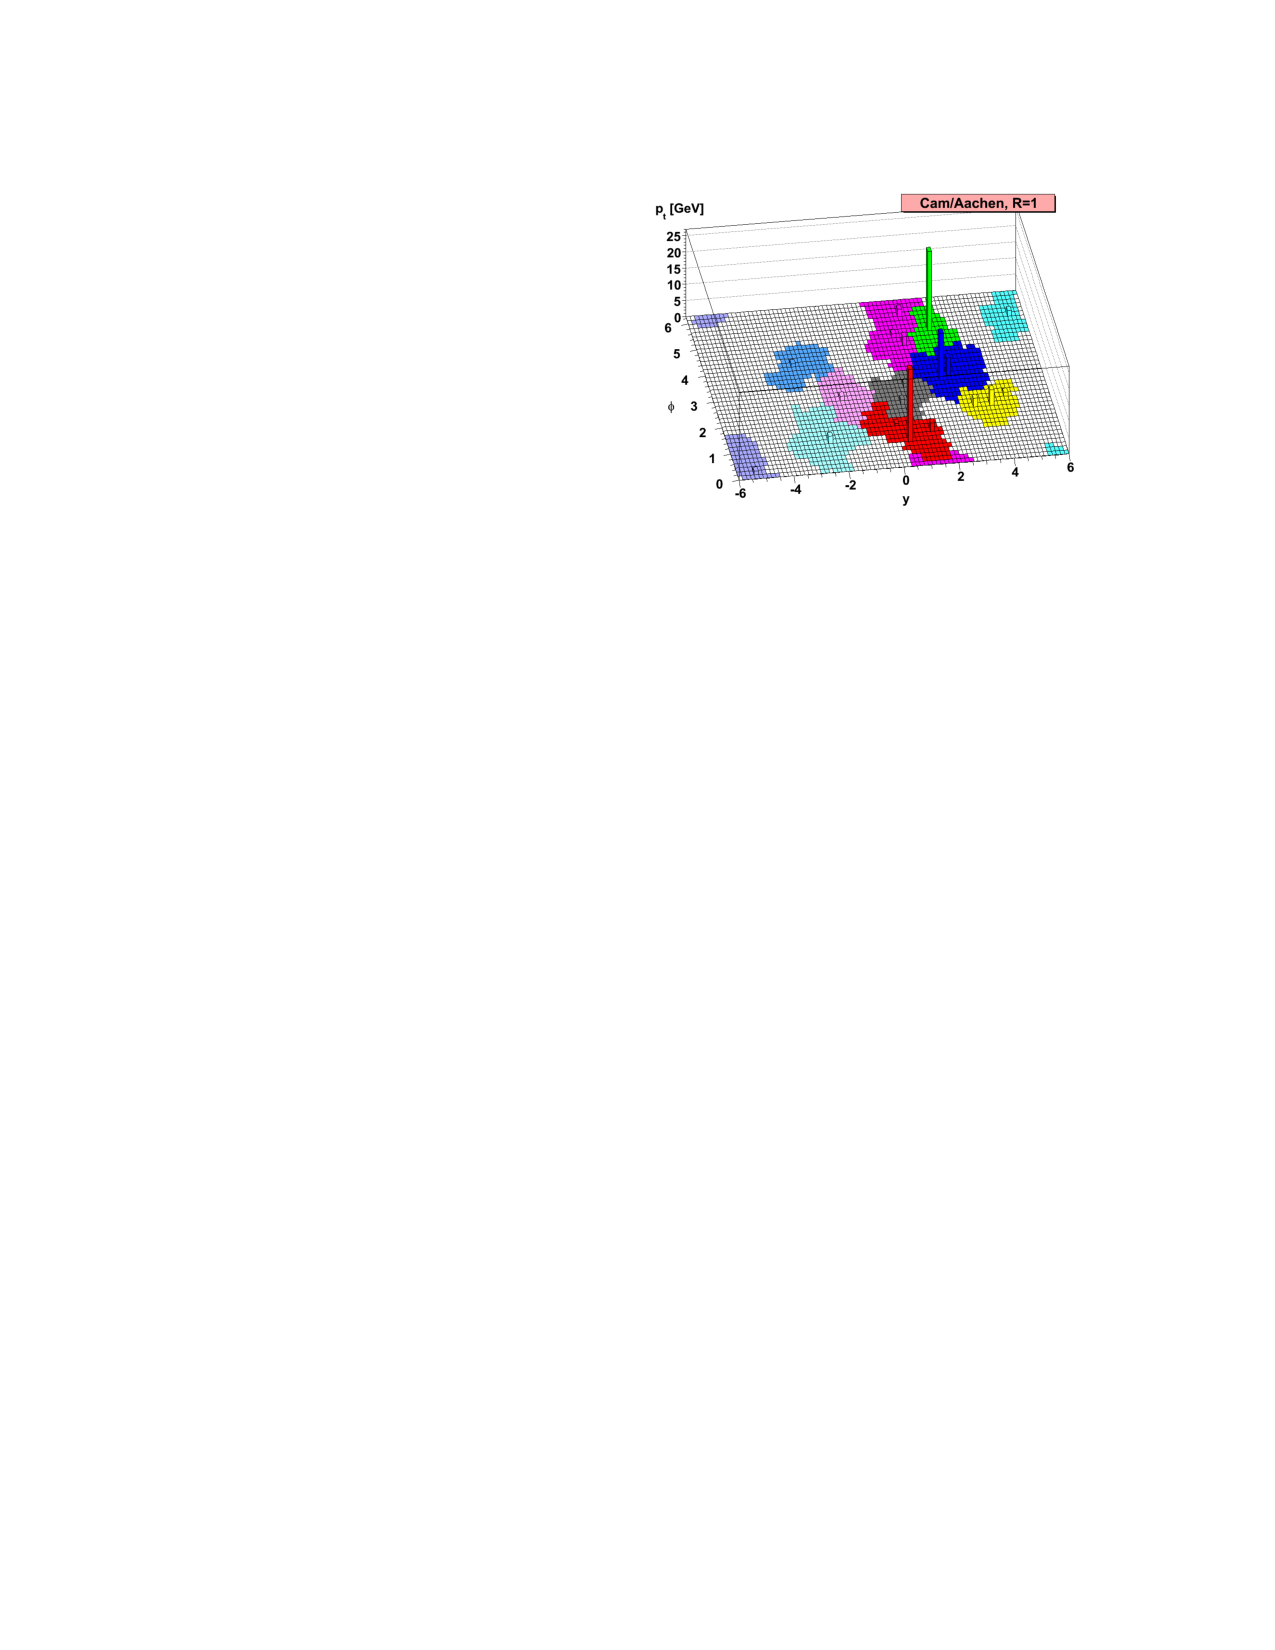
\includegraphics[width=.3\textwidth]{jetMeasurements/jetReco_CA}\hfill
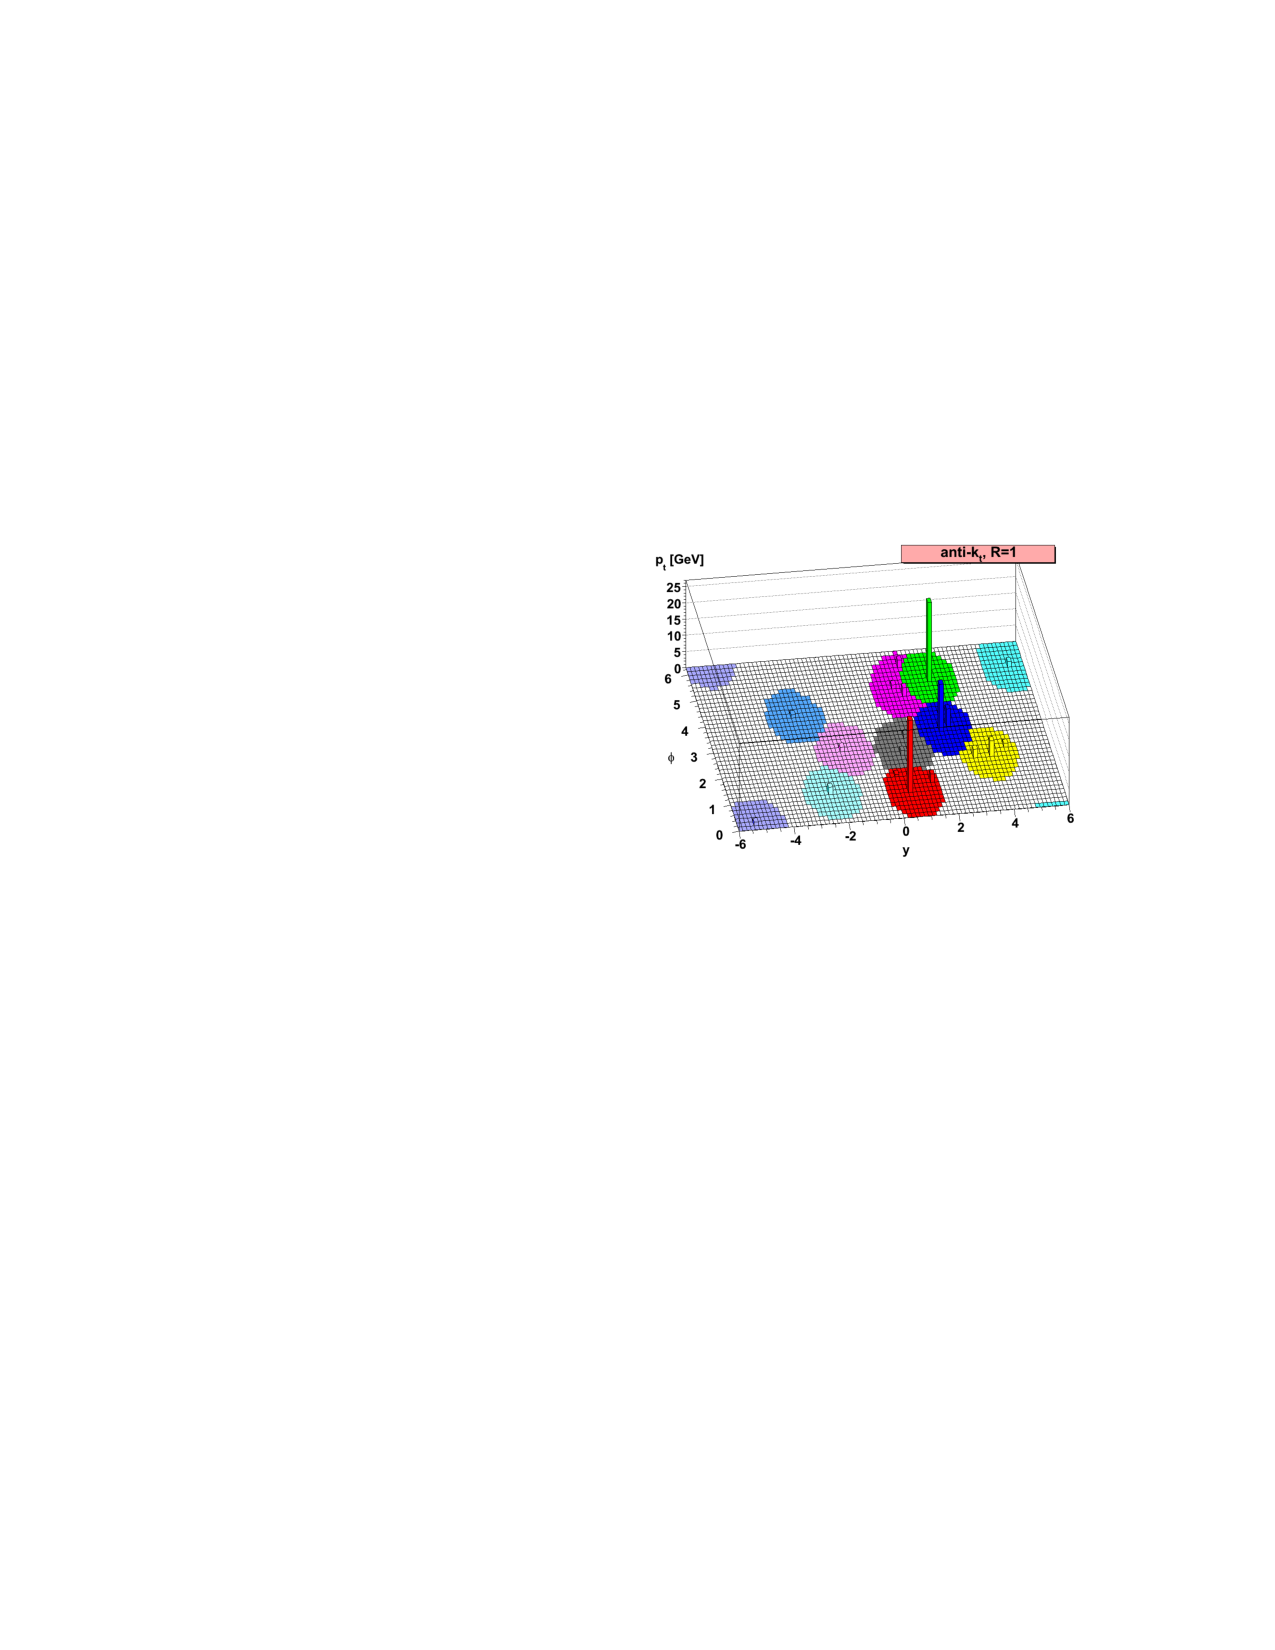
\includegraphics[width=.3\textwidth]{jetMeasurements/jetReco_antikt}\hfill
\caption{Different clustering algorithms applied to the sample parton-level event. Figure taken from \cite{Cacciari:2008gp}.}
\label{fig:JetClustering}
\end{figure}

The popularity of the \antikt\ algorithm comes from its overcoming of two common problems: collinear and infrared safety. These are related to instabilities in the cones that are found due to soft radiation. 

Figure~\ref{fig:collinearSafe} describes the collinear safety problem. In a collinear safe jet algorithm, the presence of a virtual loop or a collinear splitting of a central particle would not change the number of jets being reconstructed. On the other hand, while a collinear unsafe jet algorithm would not change its output with the presence of a virtual loop, a splitting in the central particle would lead to the left and right most particles forming individual seeds, implying two reconstructed jets \cite{Salam:2009jx}.

\begin{figure}[htp]
\centering
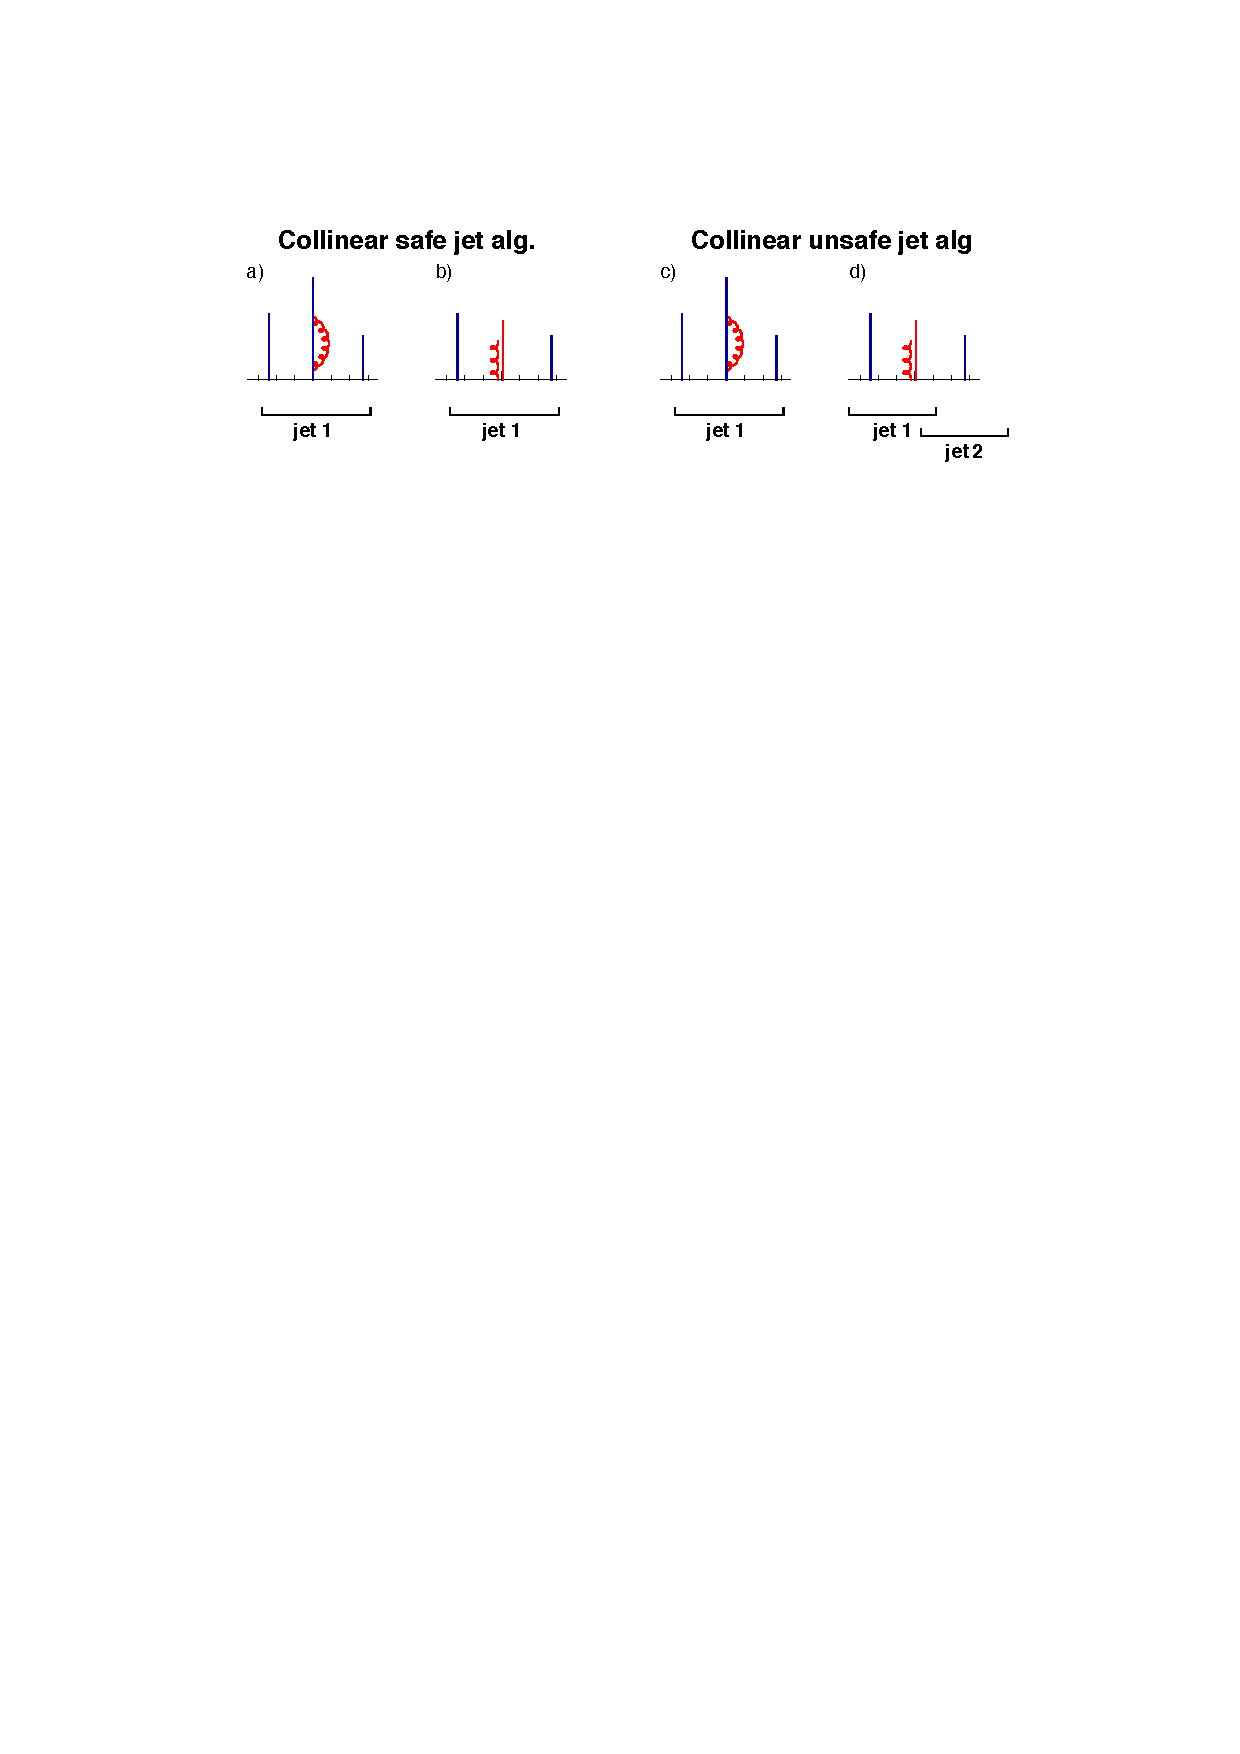
\includegraphics[width=.75\textwidth]{jetMeasurements/collinearSafe}
\caption{An illustration of collinear unsafe behavior. The particle \pt\ is proportional to the height and the horizontal axis indicates rapidity. Taken from \cite{Salam:2009jx}. }
\label{fig:collinearSafe}
\end{figure}


A schematic describing infrared un-safety is shown in Figure~\ref{fig:infraredSafe}. Here an infrared safe algorithm would use the three particles as seeds iteratively find two stable cones. An unsafe algorithm however would find three overlapping cones based on the addition of a soft seed.

\begin{figure}[htp]
\centering
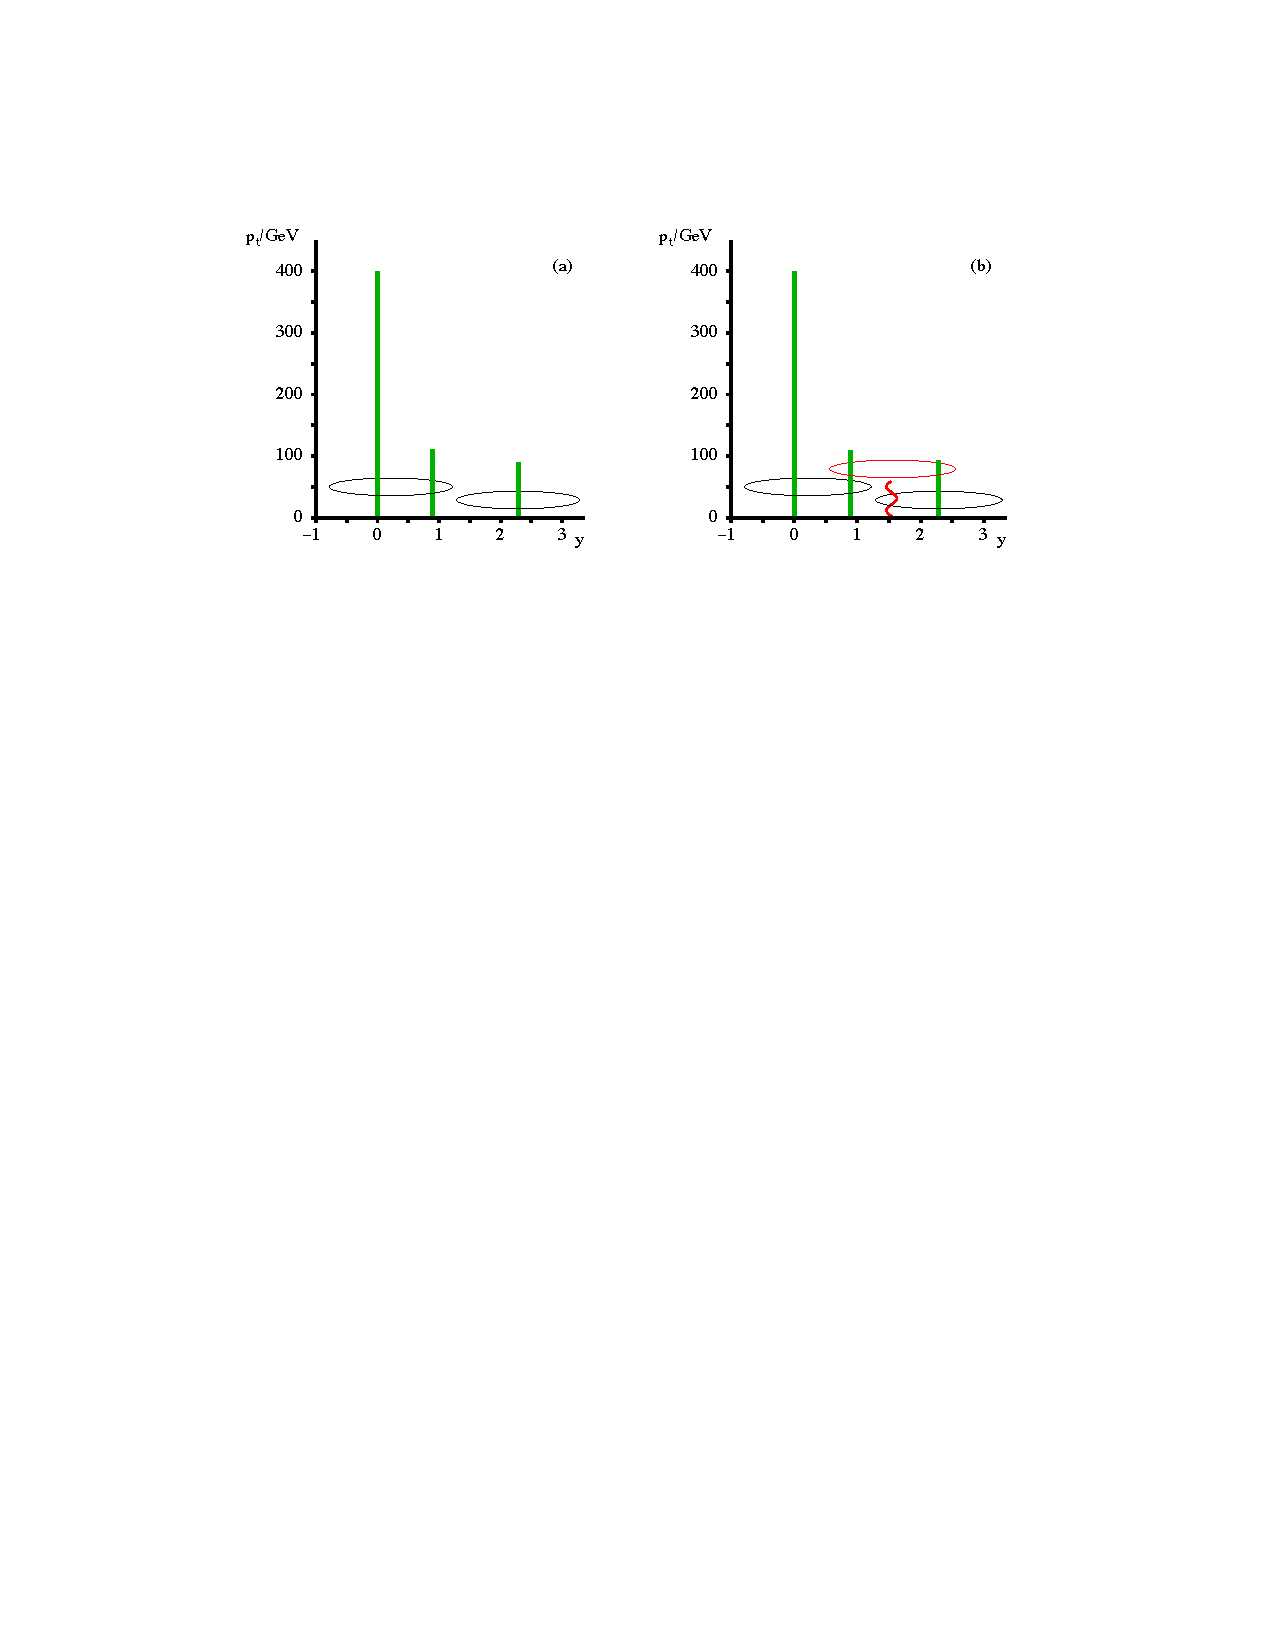
\includegraphics[width=.65\textwidth]{jetMeasurements/infraredSafe}
\caption{An illustration of infrared unsafe behavior. The particle \pt\ is proportional to the height and the horizontal axis indicates rapidity. Taken from \cite{Salam_2007} }
\label{fig:infraredSafe}
\end{figure}

% the \antikt\ reconstruction algorithm is used with the distance parameter $R=0.4$

For heavy ion collisions in ATLAS, the inputs to the algorithm are the $\eta \times \phi = 0.1 \times 0.1$ calorimeter towers. The tower energies are determined by summing up the energies of the individual calorimeter cells. The \antikt\ algorithm is first run with the distance parameter $R=0.2$, following which an underlying event subtraction procedure is performed. A first estimate of the average underlying event energy density $\rho_i (\eta)$ is done in 0.1 slices of $\eta$ in each calorimeter layer $i$ after excluding the regions that overlap with the seed jets. A modulation of $2v_{2} \cos[2(\phi-\Psi_2)] $ is applied to account for the flow from the QGP and the underlying event is subtracted to give $E_{Tj}^{\mathrm{sub}}$:

\begin{align}
E_{Tj}^{\mathrm{sub}} = E_{Tj} - A_j \rho_i (\eta_j) 1+2v_{2i} \big(\cos[2(\phi-\Psi_2)] \big)
\end{align}
where $ E_{Tj} , \eta_j, \phi_j$ and $A_j$ are the cell $E_T, \eta, \phi$ and area for cell $j$ in layer $i$. This process is done iteratively done one more time after getting new seeds with the distance parameter $R = 0.2$ and excluding areas that are within $\Delta R = 0.4$ of the seeds. Updated values of $\rho{'}_i$ and $v{'}_2$ are recalculated and used to estimate the background that is subtracted from the original cell energies. More details on this procedure can be found in \cite{2013220}.



%A few jet measurements and their modifications by the presence of the Quark Gluon Plasma are discussed in Section~\ref{sec:jetMeasurements}.
%

%%%%%%%%%%%%%%%%%%%%%%%%%%%%%%%%%%%%%%%%%%%%%%%%
%  jet cross section in  \sqrts = 13 TeV \pp\ collisions can be seen in Figure~\ref{fig:incljetCS}
%
%
%
%\begin{figure}[htbp]
%\begin{center}
%\includegraphics[width=0.55\textwidth]{figures/theory/incljetCS}
%\caption{The inclusive jet cross section as a function of \pt\ and $|y|$ as measured by ATLAS. The data are compared to NLO pQCD calculations. Taken from \cite{Aaboud:2017wsi}}
%\label{fig:incljetCS}
%\end{center}
%\end{figure}
%
%
%
%
%

%
%\begin{figure}[htbp]
%\begin{center}
%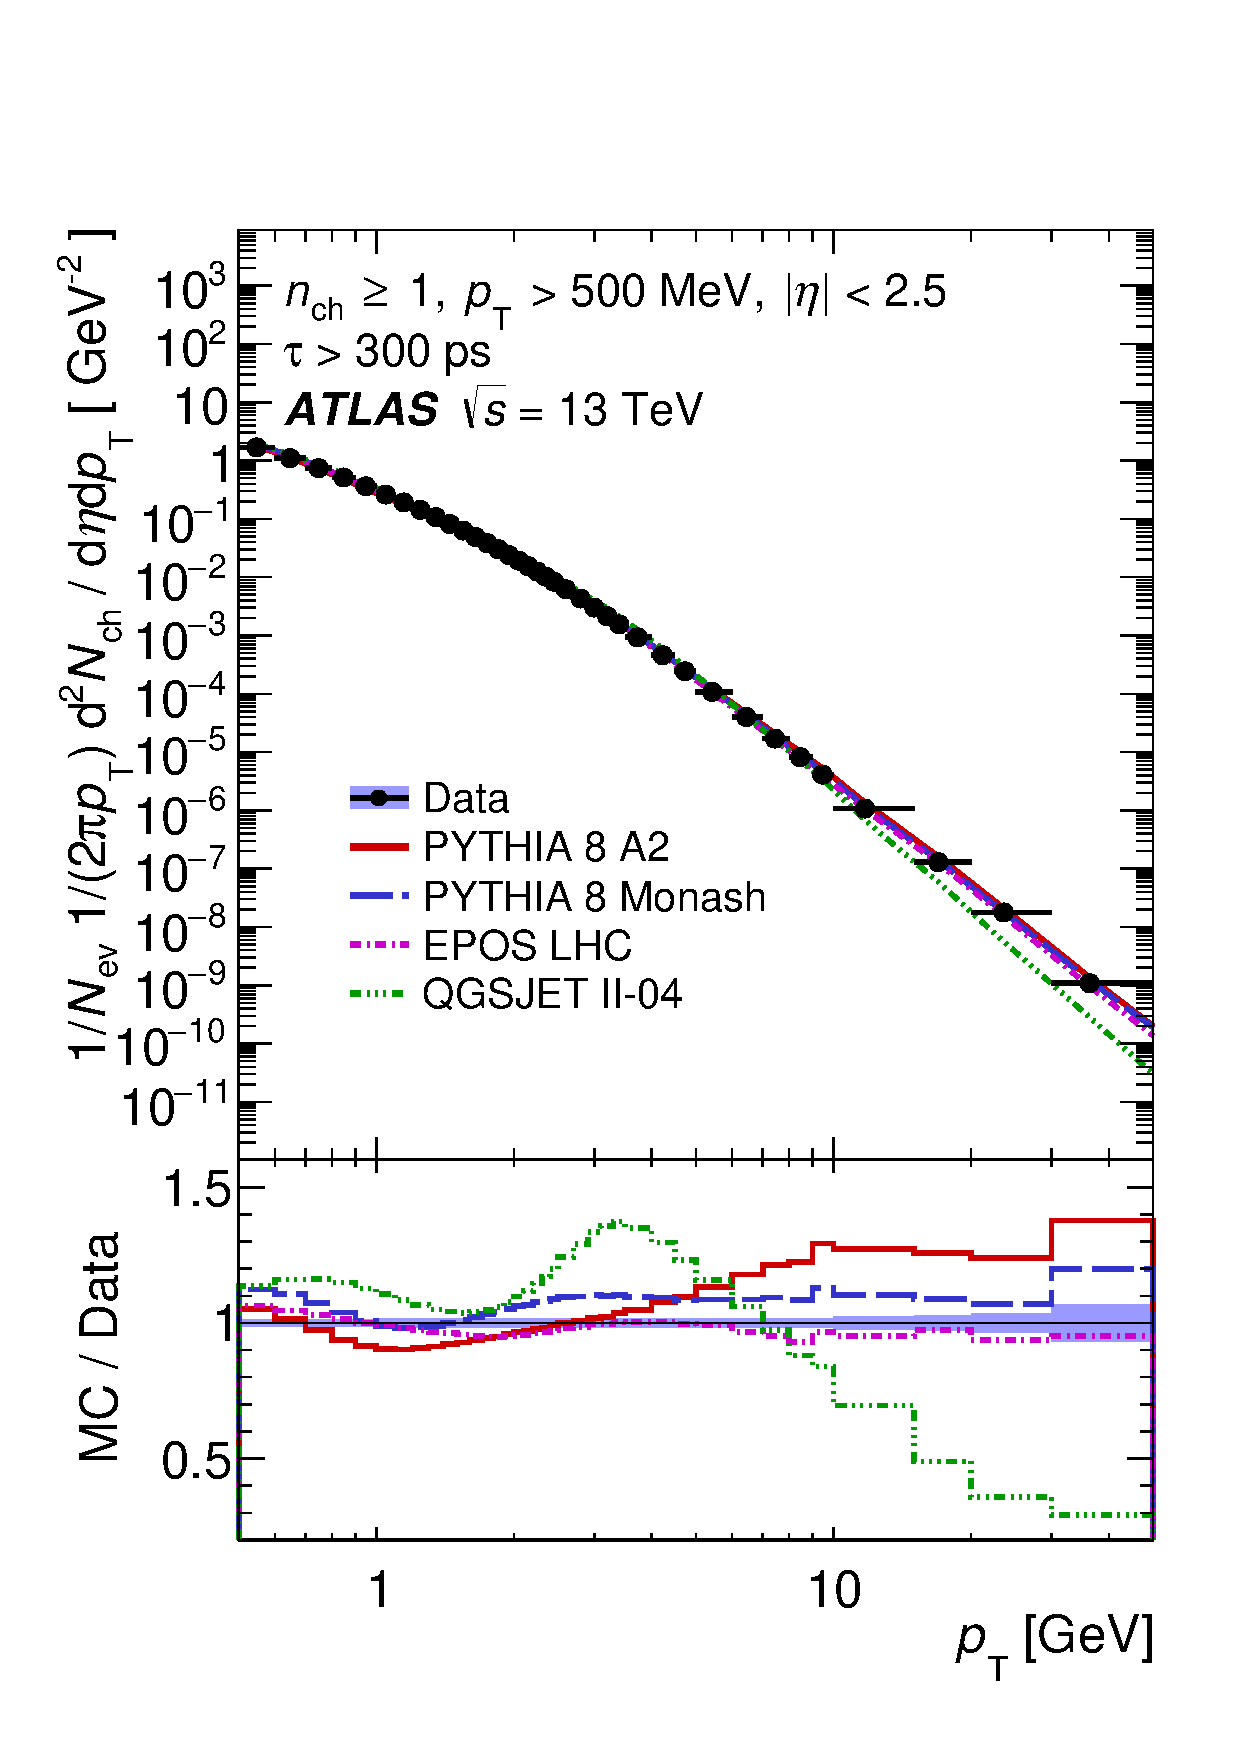
\includegraphics[width=0.55\textwidth]{figures/theory/inclhadronCS}
%\caption{The charged particle multiplicities as a function of transverse momentum \pt\ in \sqrts = 13 TeV \pp\ collisions as measured by ATLAS. The data are compared to NLO pQCD calculations. Taken from \cite{201667}. }
%\label{fig:inclhadronCS}
%\end{center}
%\end{figure}
%
%
%
%Equation~\ref{eq:hadronCS} is written at leading order (LO) and includes contributions from $2\rightarrow2$ cross sections, LO re-summed PDFs and FFs, and single loop expression for the strong coupling \alphas. At next to leading order (NLO), the contributions from real $2\rightarrow3$ and virtual $2\rightarrow3$ processes, as well as the double loop expression for \alphas are included. These calculations describe the inclusive and pQCD, NLO calculations have next to leading order (NLO) calculations that include Figure~\ref{fig:incl_hadron_CS} hows the inclusive jet cross section as measured by ATLAS in \sqrts = 13 TeV \pp\ collisions. 
%
%
%
%
%In a heavy ion collision where the QGP is formed, the hard scattering interactions between the partons strongly interact with the QGP due to their color charge and are modified and lose energy via collisions with the medium constituents, or gluon bremsstrahlung. 
